\addcontentsline{toc}{section}{Introduction}
\section*{Introduction}
Ce chapitre s'attelle à la présentation du prototype de StudX, l’application de communication en temps réel que nous proposons. 
Nous en présenterons les diverses fonctionnalités accompagnées de capture d'écran. 
Puis, au travers d’une discussion, nous en présenterons les limites, les contraintes et les possibilités d’expansion.

\section{Résultats}
\subsection{Authentification}
L'accès à l’application est subordonné à l'authentification de l’utilisateur. 
La figure \ref{fig:proto_auth} en présente l’interface. 
Elle offre la possibilité de se connecter ou de s'inscrire.

\begin{figure}[H]
  \centering
  \frame{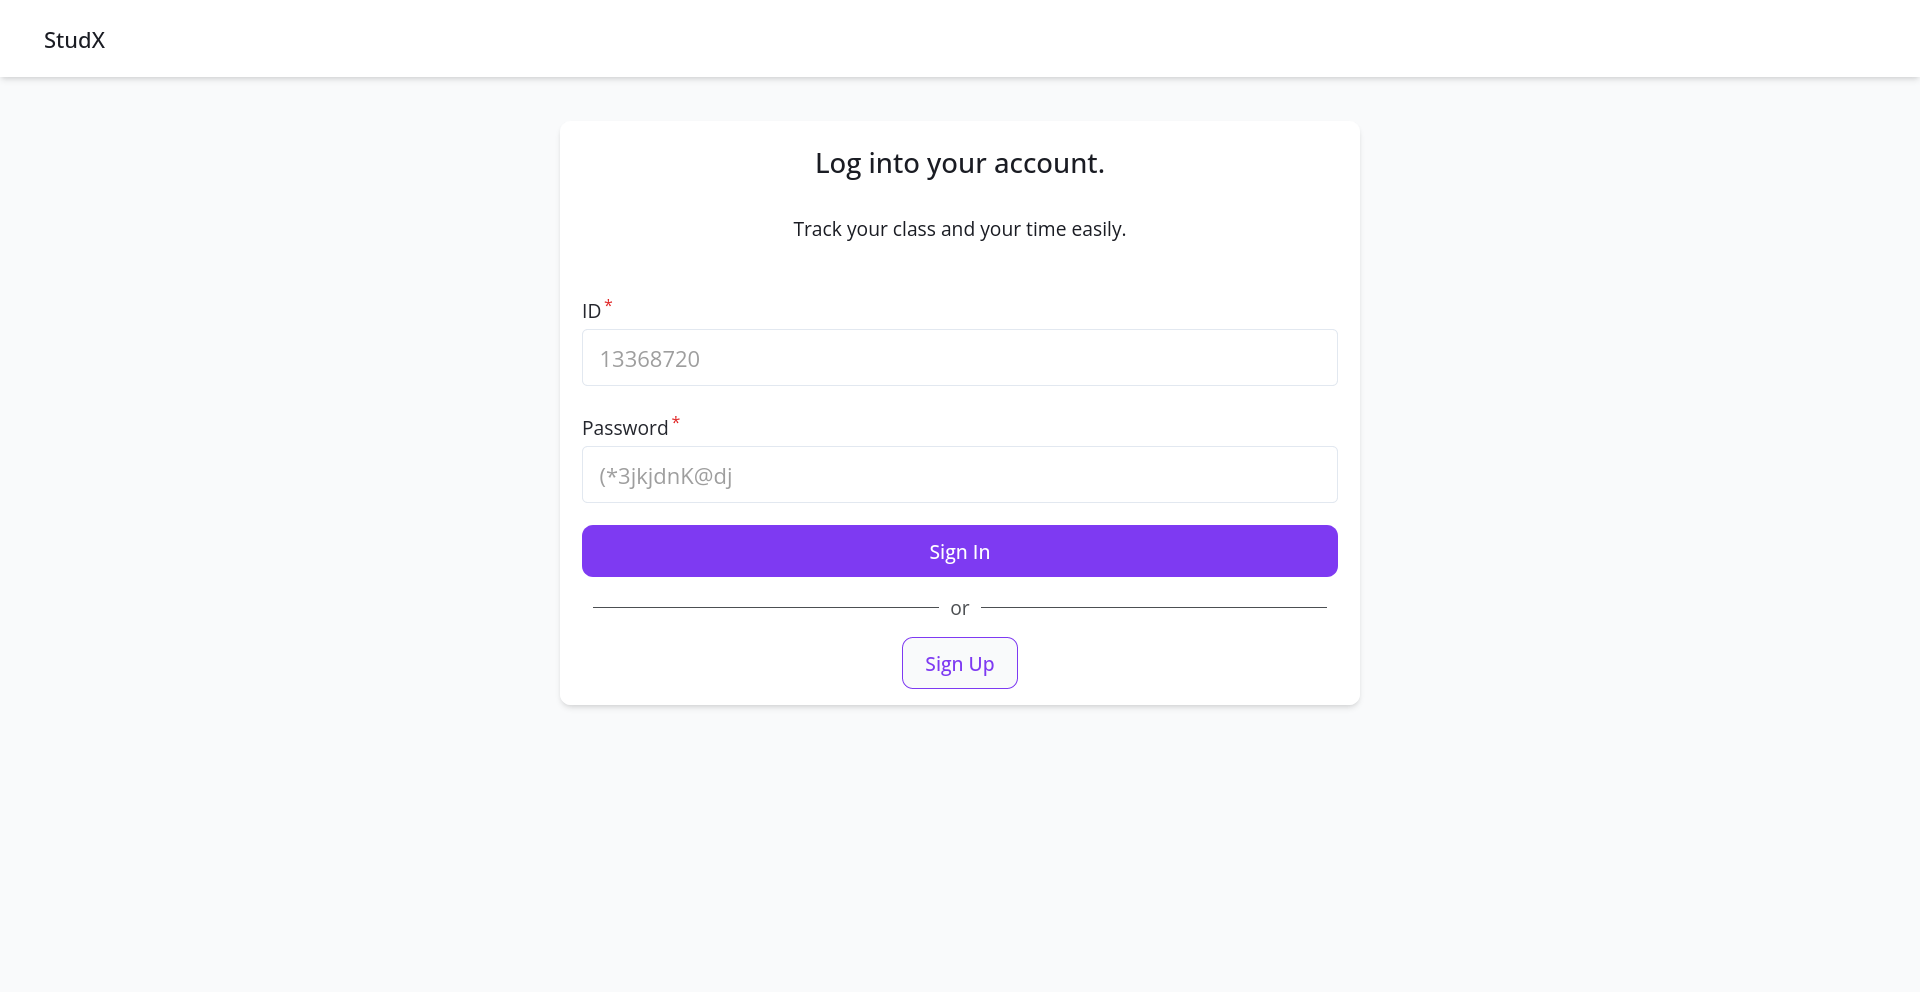
\includegraphics[width=0.95\textwidth]{prototype/login}}
  \caption{Page d'authentification de \textbf{StudX}}
  \label{fig:proto_auth}
\end{figure}

\subsection{Calendrier}
Après authentification, l’utilisateur accède au calendrier des divers événements planifiés. 
Il lui est possible de réduire ou d'étendre la vue au jour actuel, aux semaines ou encore aux mois.  
S’il s’agit d’un administrateur ou d’un enseignant, il peut en ajouter de nouveaux.
La figure \ref{fig:proto_calendar_view} présente le calendrier,qui présente tous les programmes du mois courant.

\begin{figure}[H]
  \centering
  \frame{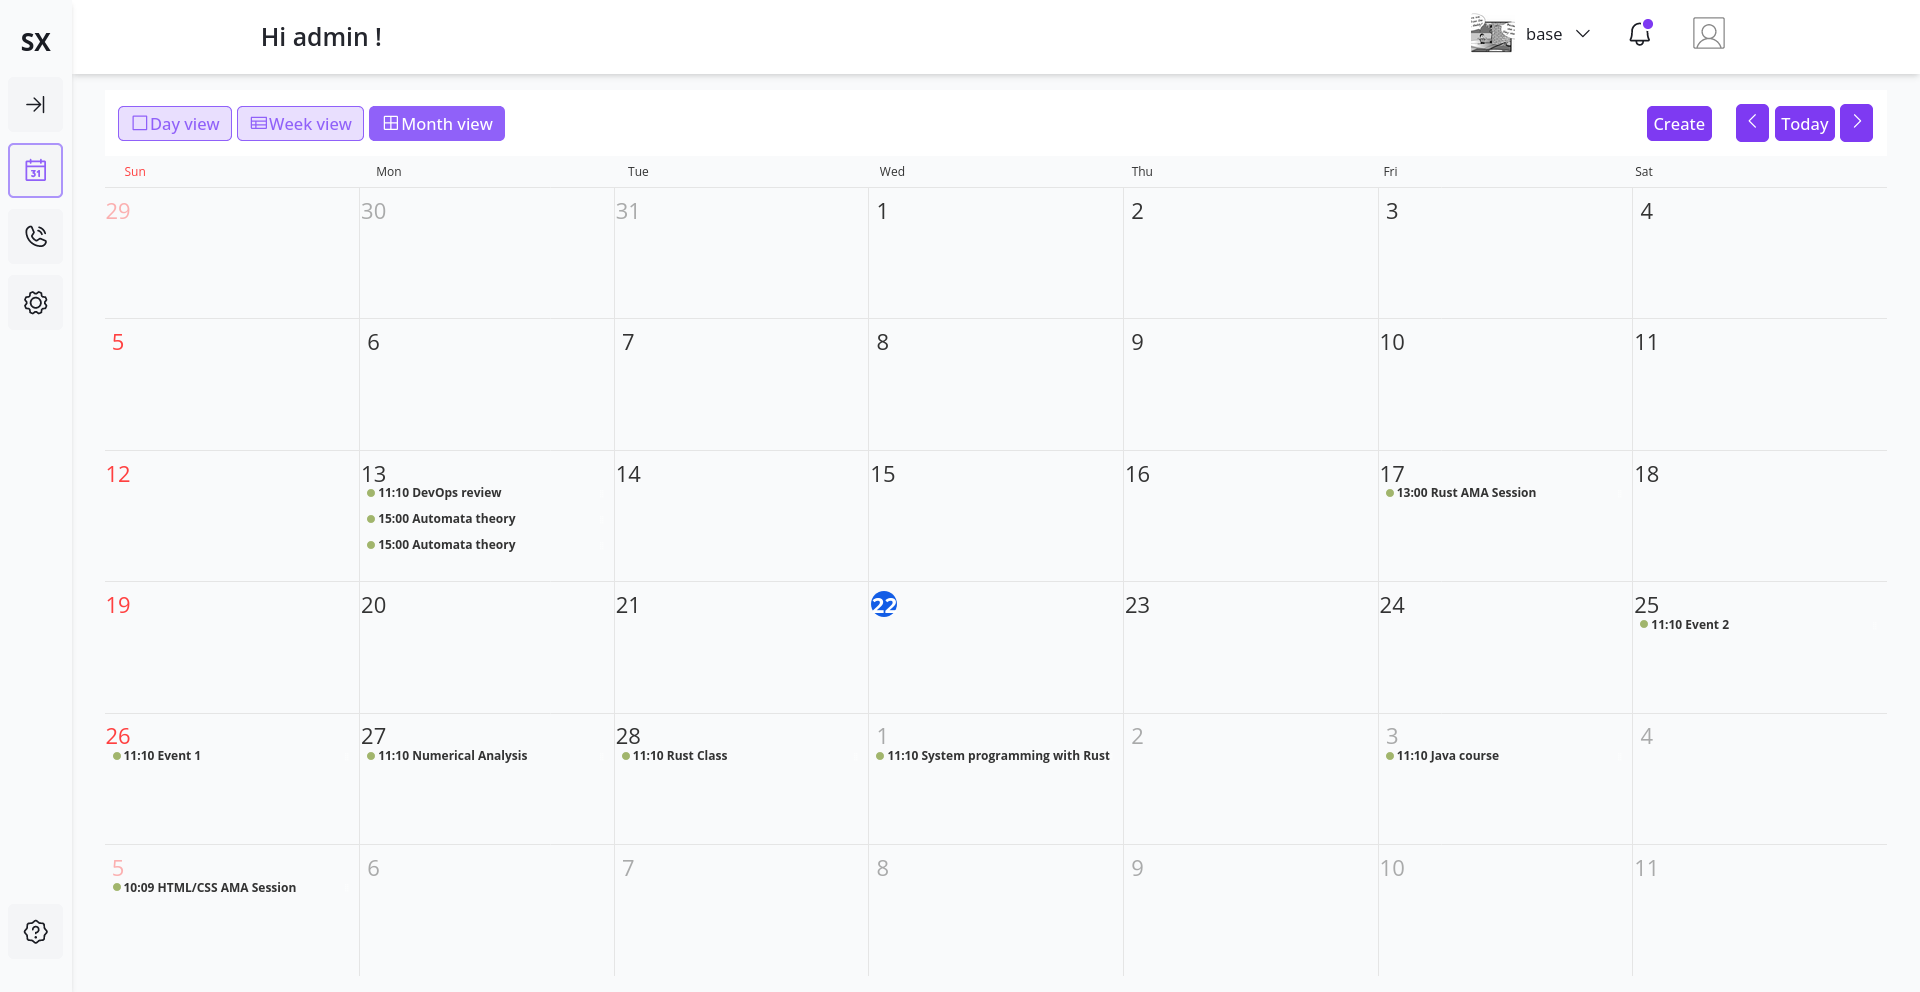
\includegraphics[width=0.95\linewidth]{prototype/calendar-view}}
  \caption{Calendrier des planifications}
  \label{fig:proto_calendar_view}
\end{figure}

S’il dispose des permissions nécessaires, 
l’utilisateur peut ajouter un événement au calendrier en suivant le formulaire que montre la figure \ref{fig:add_event}.


\begin{figure}[H]
  \centering
  \frame{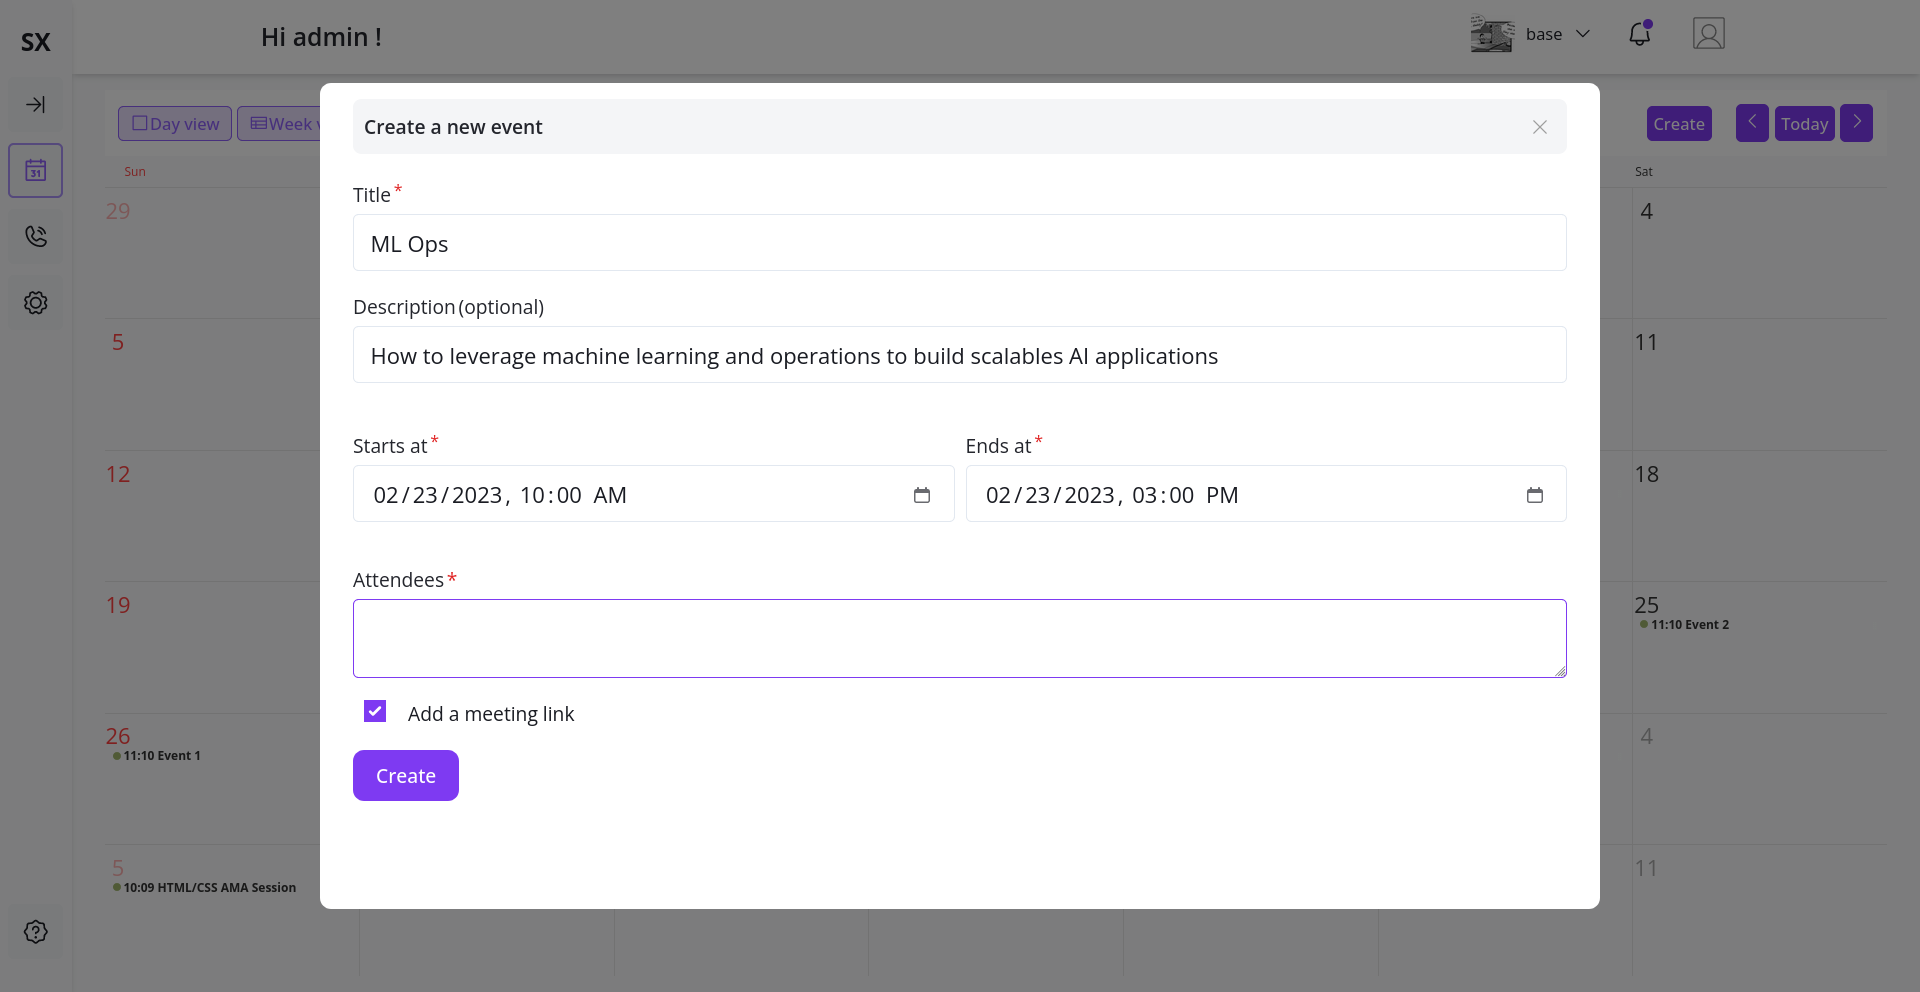
\includegraphics[width=0.825\linewidth]{prototype/add-event-form}}
  \caption{Calendrier des planifications}
  \label{fig:add_event}
\end{figure}

Il est possible d’associer à l'événement un lien d'accès à la session de conférence en ligne. 
Pour y accéder par la suite, les utilisateurs peuvent consulter les détails dudit événement (figure \ref{fig:event_details}).

\begin{figure}[H]
  \centering
  \frame{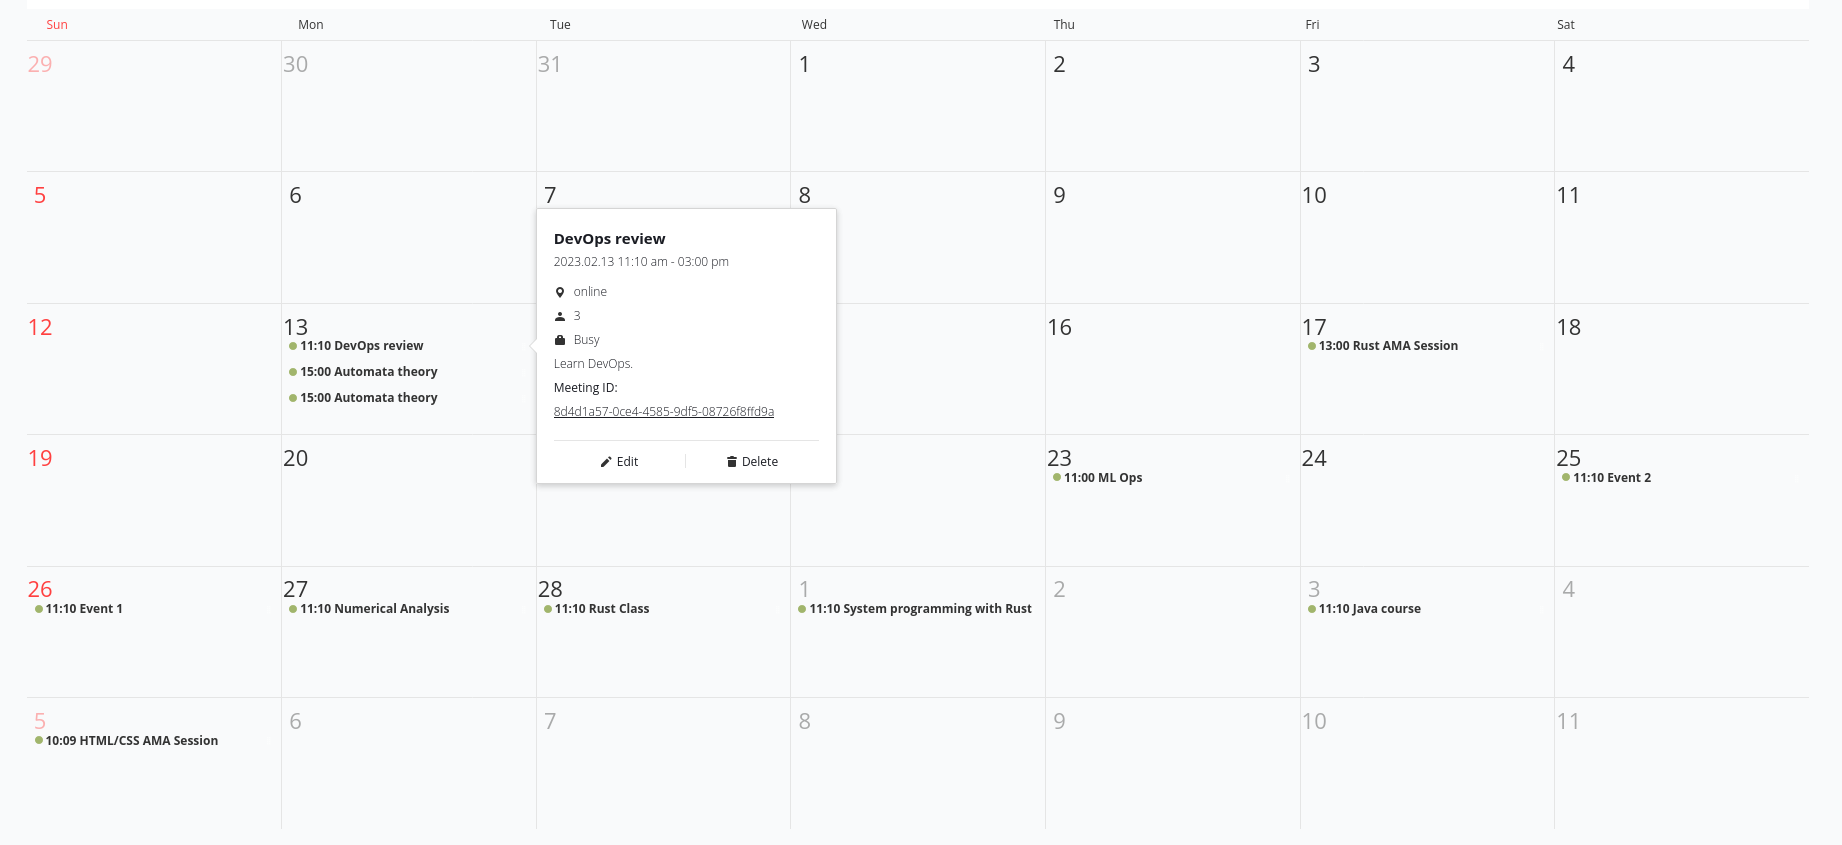
\includegraphics[width=\linewidth]{prototype/event-detail}}
  \caption{Détails d'un événement}
  \label{fig:event_details}
\end{figure}

\subsection{Sessions en ligne}
Les événements incluant un lien donnent accès à une session en ligne que
peuvent rejoindre tous les participants disposant du lien.
La figure \ref{fig:participants_grids} présente à quoi ressemble l’interface par défaut, avec la grille des participants et les options de contrôle. 
Outre la voix, les participants ont la possibilité d’interagir entre eux via des messages écrits (figure \ref{fig:room_chat}).

\begin{figure}[H]
  \centering
  \begin{subfigure}[b]{\textwidth}
      \centering
      \frame{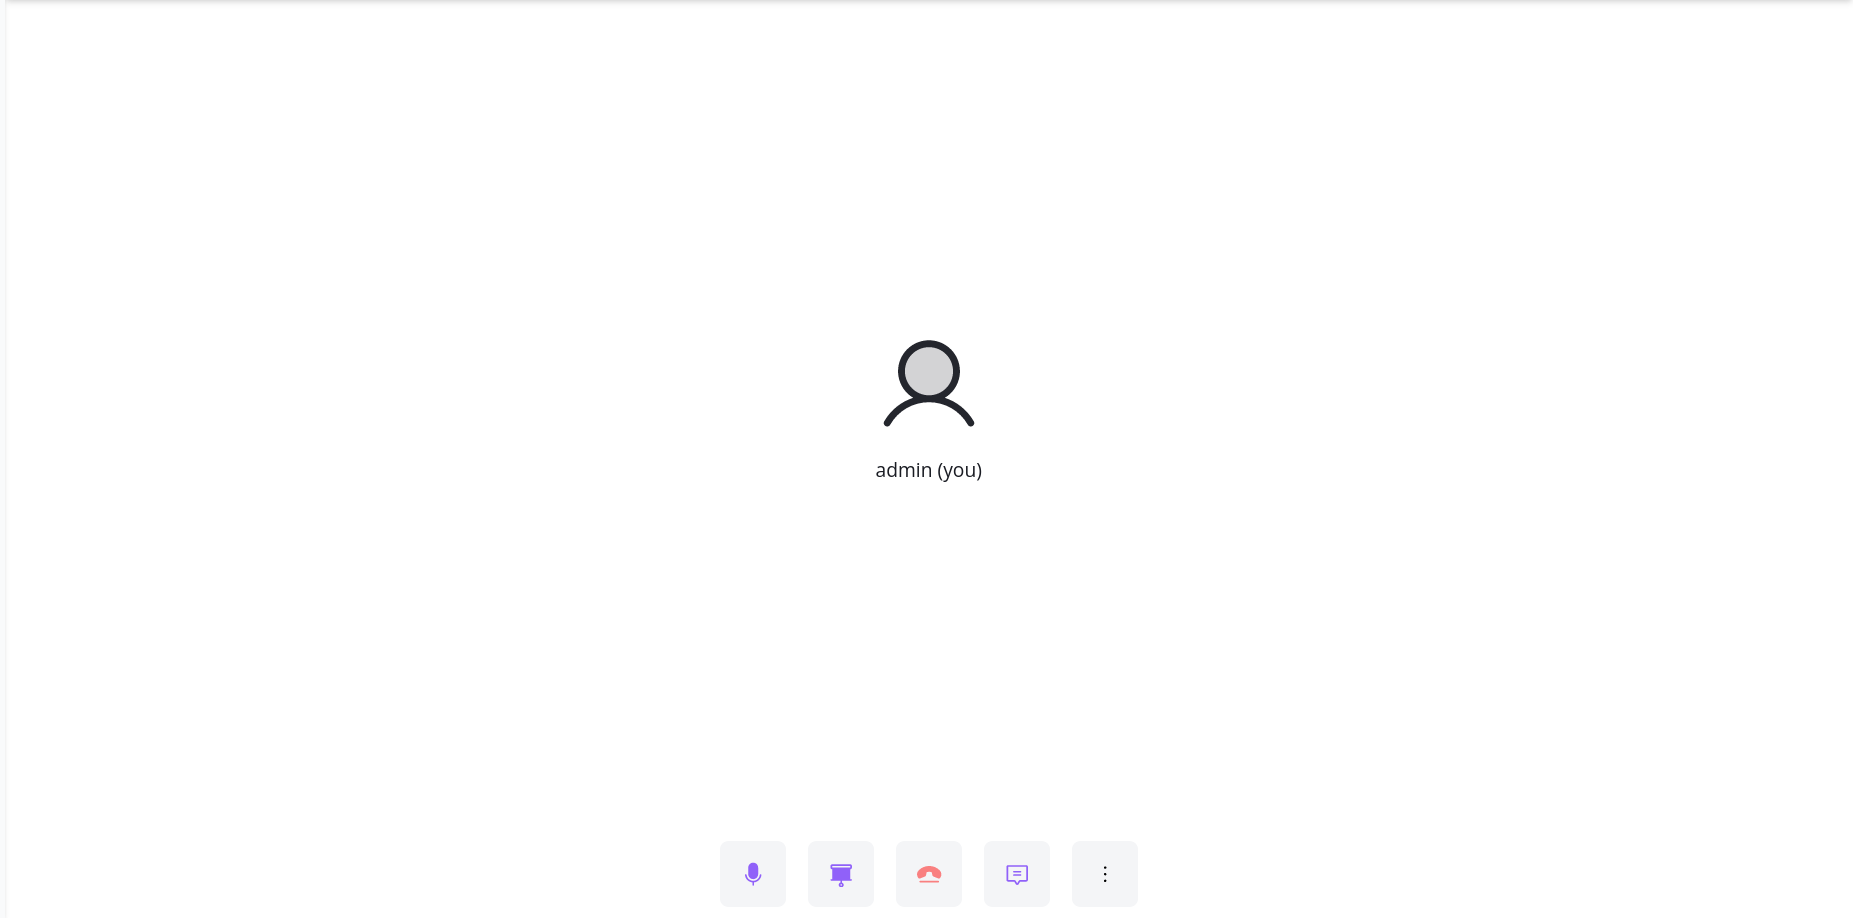
\includegraphics[width=\linewidth]{prototype/user-single-in-room}}
      \caption{Un participant}
  \end{subfigure}
  \vskip\baselineskip
  \begin{subfigure}[b]{\textwidth}
      \centering
      \frame{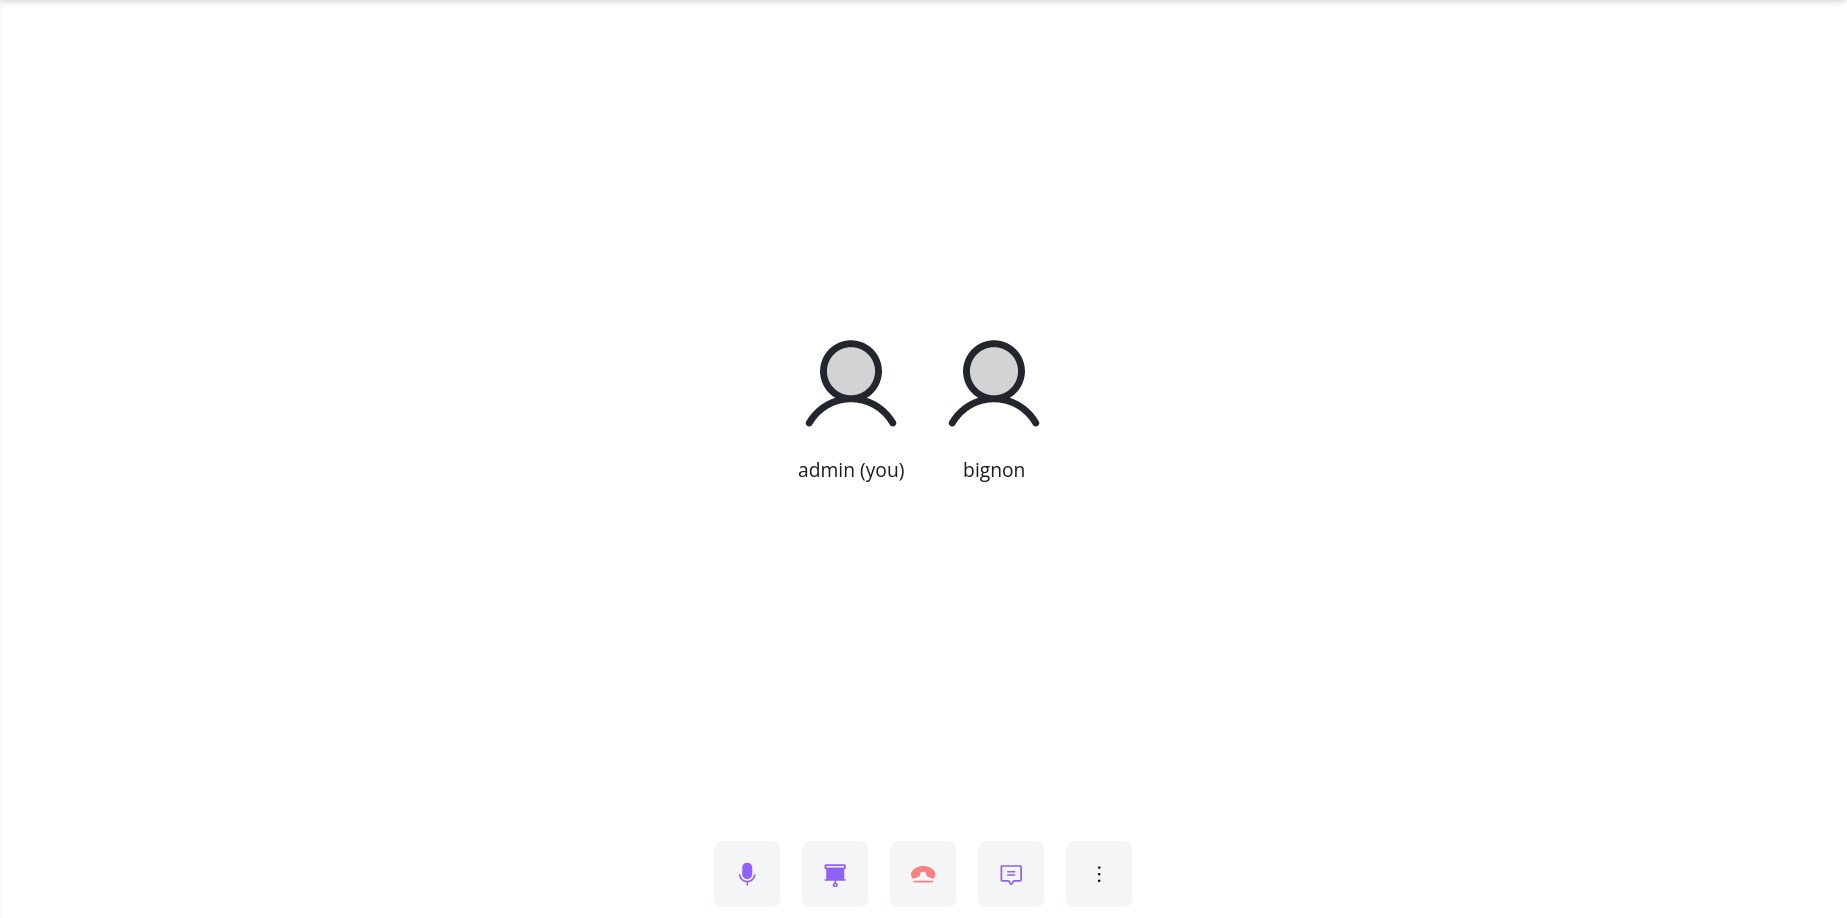
\includegraphics[width=\linewidth]{prototype/user-with-participants-in-room}}
      \caption{Deux participants}
  \end{subfigure}
  \caption{Grille des participants et boutons de contrôle.}
  \label{fig:participants_grids}
\end{figure}

\begin{figure}[H]
  \centering
  \frame{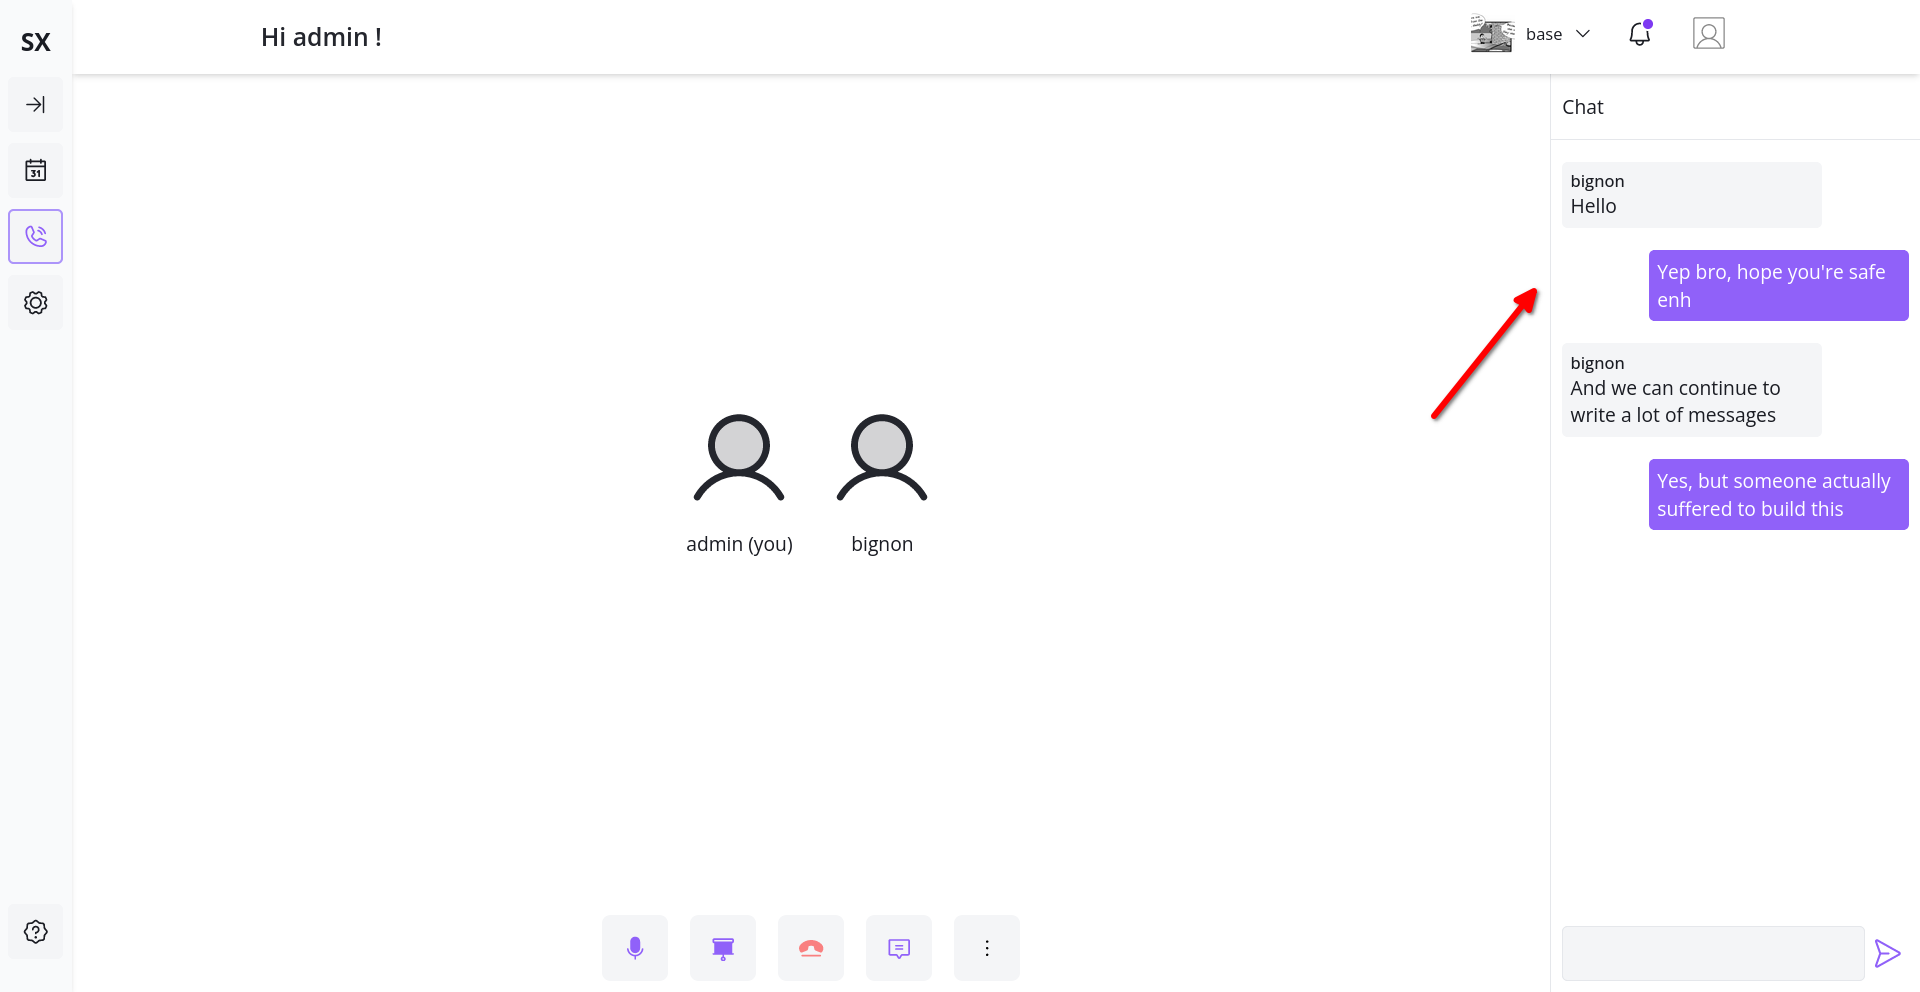
\includegraphics[width=\linewidth]{prototype/room-chat}}
  \caption{Messagerie instantannée intégrée à \textbf{StudX}}
  \label{fig:room_chat}
\end{figure}

Plusieurs autres fonctionnalités sont exploitables. 
L’une d’elles est le partage d'écran. Pour illustrer, nous nous sommes servis de deux appareils avec 
l’un faisant le partage, comme le montre la figure \ref{fig:screenshare}.


\begin{figure}[H]
  \centering
  \begin{subfigure}[b]{\textwidth}
      \centering
      \frame{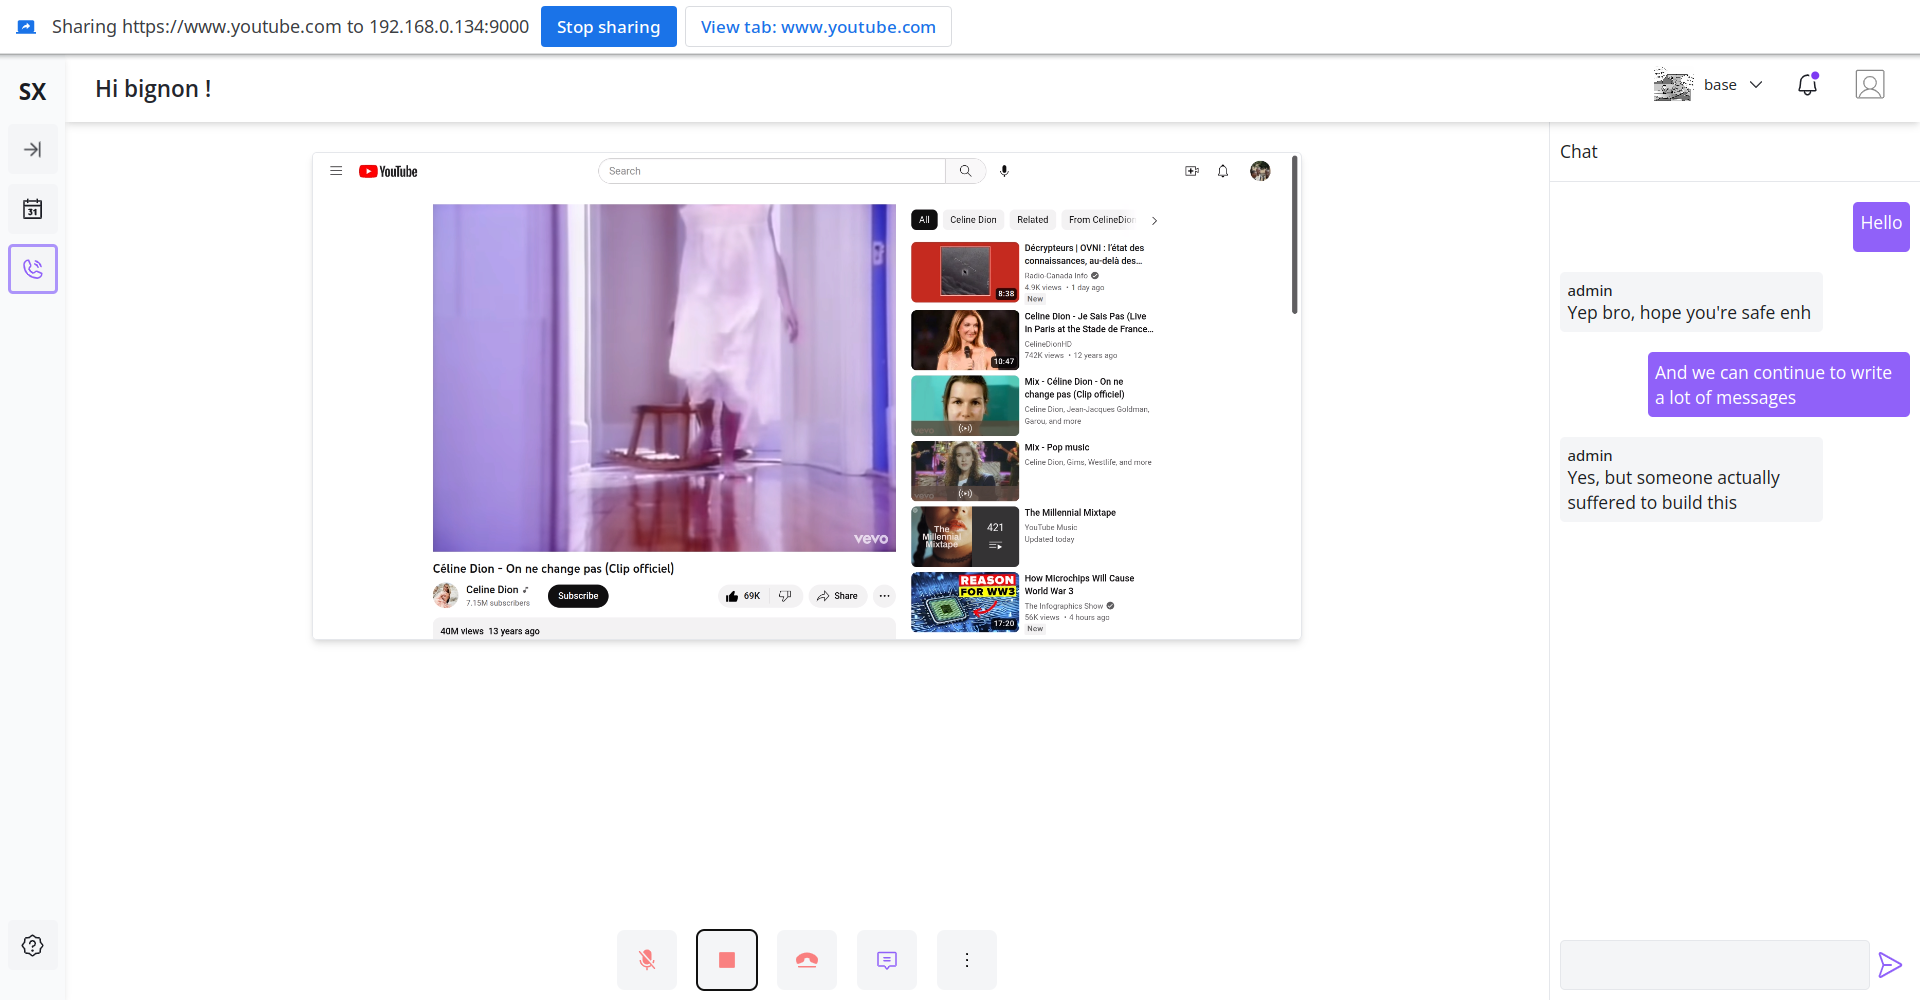
\includegraphics[width=\linewidth]{prototype/user-sharing-screen}}
      \caption{Participant faisant un partage d'écran.}
  \end{subfigure}
  \vskip\baselineskip
  \begin{subfigure}[b]{\textwidth}
      \centering
      \frame{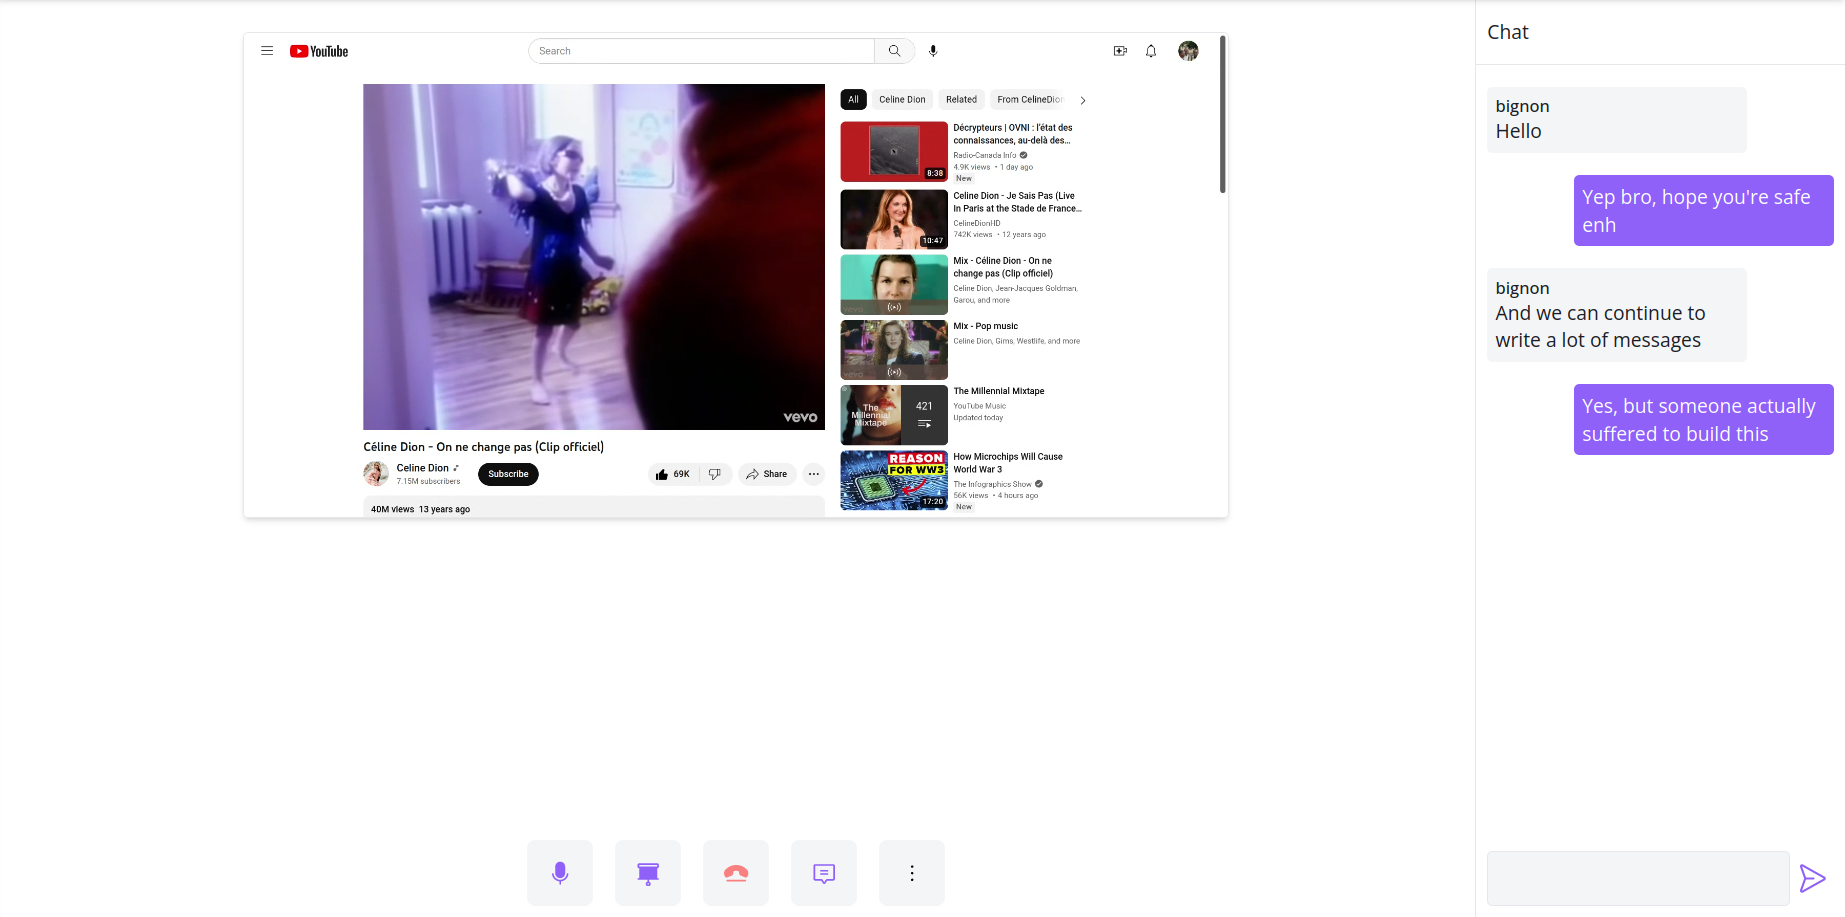
\includegraphics[width=\linewidth]{prototype/user-viewing-screen}}
      \caption{Visualisation du partage d'écran}
  \end{subfigure}
  \caption{Partage d'écran.}
  \label{fig:screenshare}
\end{figure}

Les participants disposent également d’un whiteboard, 
c'est-à- dire un tableau virtuel, pour effectuer des illustrations. 
Le contenu est synchronisé entre tous les participants. 
La figure \ref{fig:whiteboard} fait une démonstration de ladite fonction.

\begin{figure}[H]
  \centering
  \frame{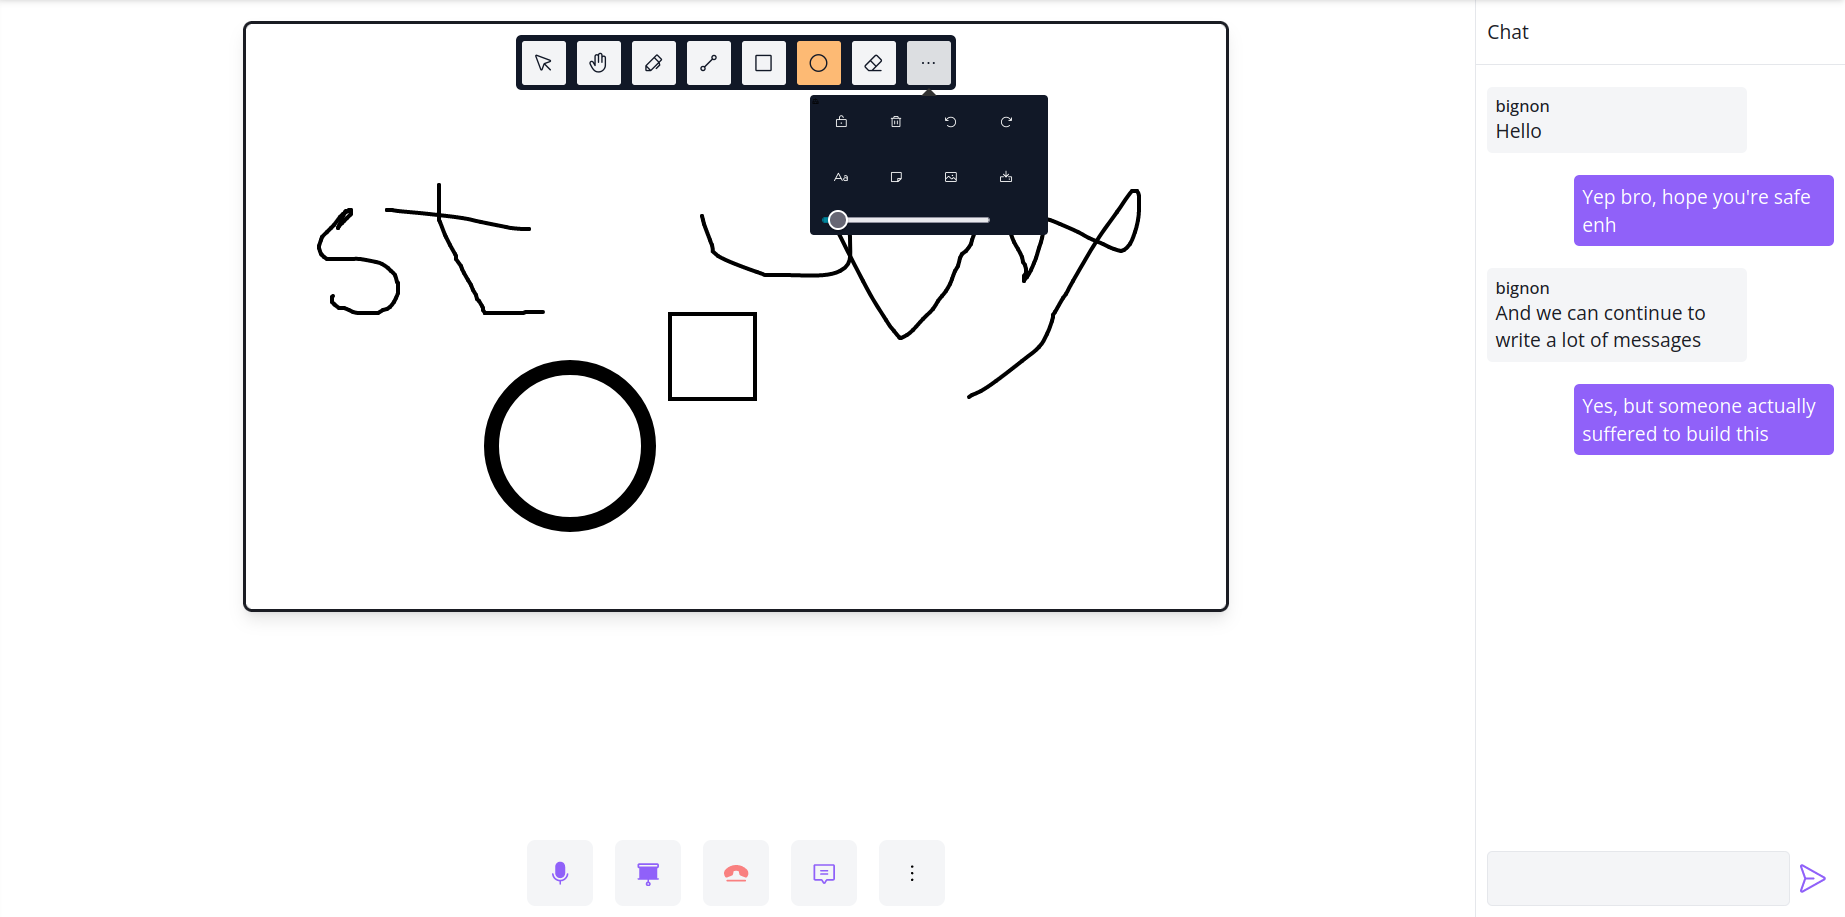
\includegraphics[width=\linewidth]{prototype/whiteboard}}
  \caption{Tableau virtuel}
  \label{fig:whiteboard}
\end{figure}

On peut également percevoir sur l’image, les modifications apportées au projet Open Source qui a servi de base au développement de cette fonctionnalité.
L’application dispose également d’un dispositif de notes intégré, que nous qualifions de \textbf{Writepad}. La figure \ref{fig:writepad} en fait la présentation.


\begin{figure}[H]
  \centering
  \frame{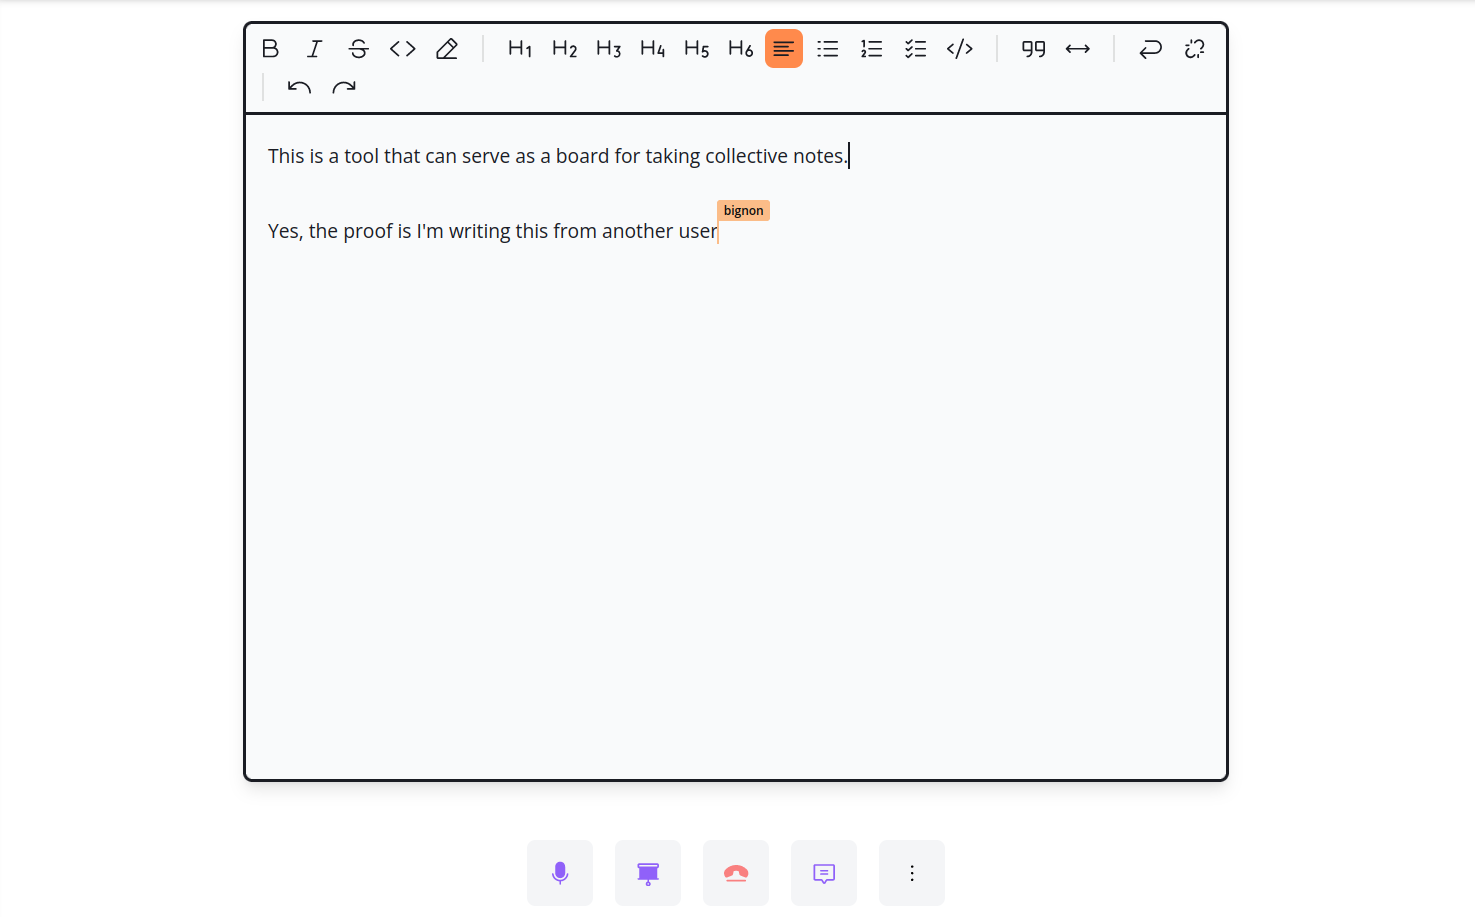
\includegraphics[width=\linewidth]{prototype/wrritepad}}
  \caption{Outil de note synchronisé}
  \label{fig:writepad}
\end{figure}

Les fonctions suscitées rendent inaccessible la grille des participants. 
Mais il est toujours possible de pourvoir y accéder dans la même section que la messagerie, comme le montre la figure \ref{fig:participants_aside}.

\begin{figure}[H]
  \centering
  \frame{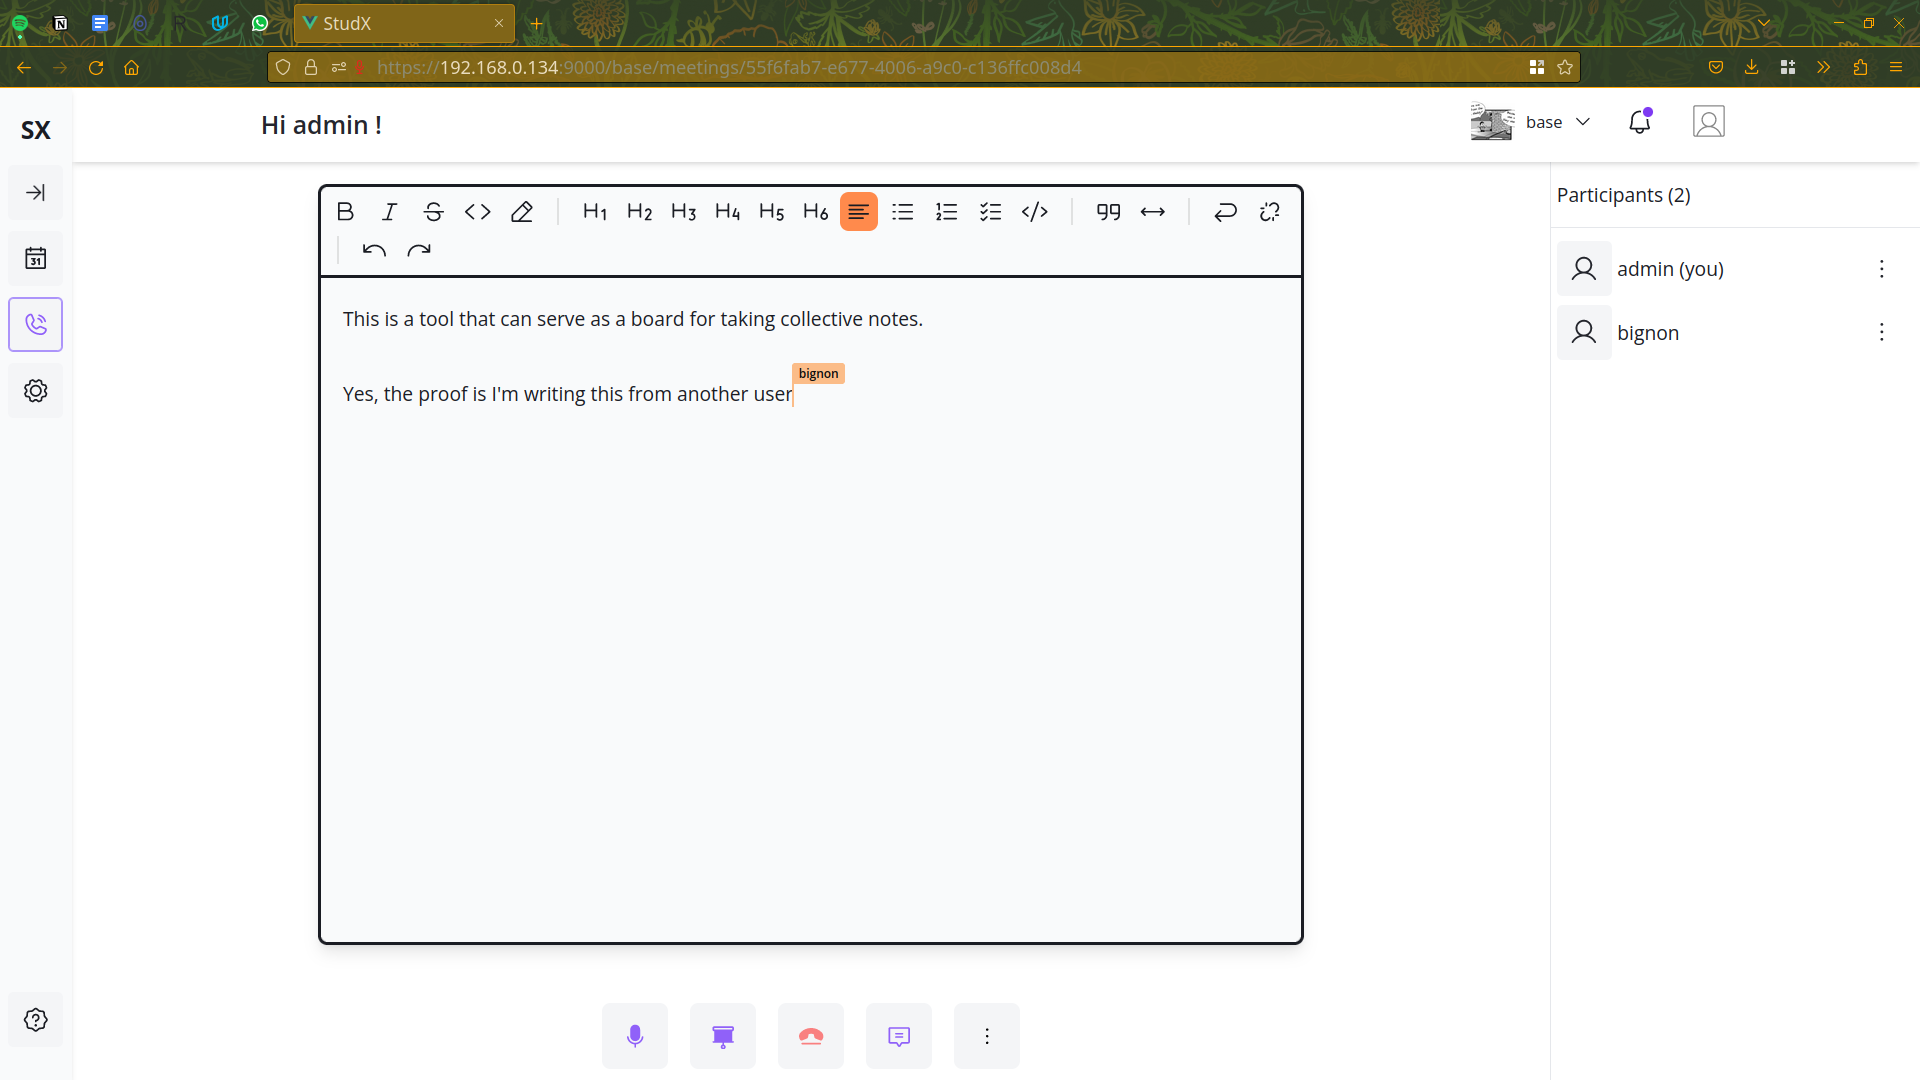
\includegraphics[width=\linewidth]{prototype/participants}}
  \caption{Liste des participants}
  \label{fig:participants_aside}
\end{figure}

Enfin, chaque utilisateur a la possibilité de quitter la réunion. Si par mégarde, il essaie de recharger par exemple, l’onglet, une confirmation est requise (si le navigateur supporte cette fonctionnalité), comme le montre la figure \ref{fig:exit}.

\begin{figure}[H]
  \centering
  \begin{subfigure}[b]{\textwidth}
      \centering
      \frame{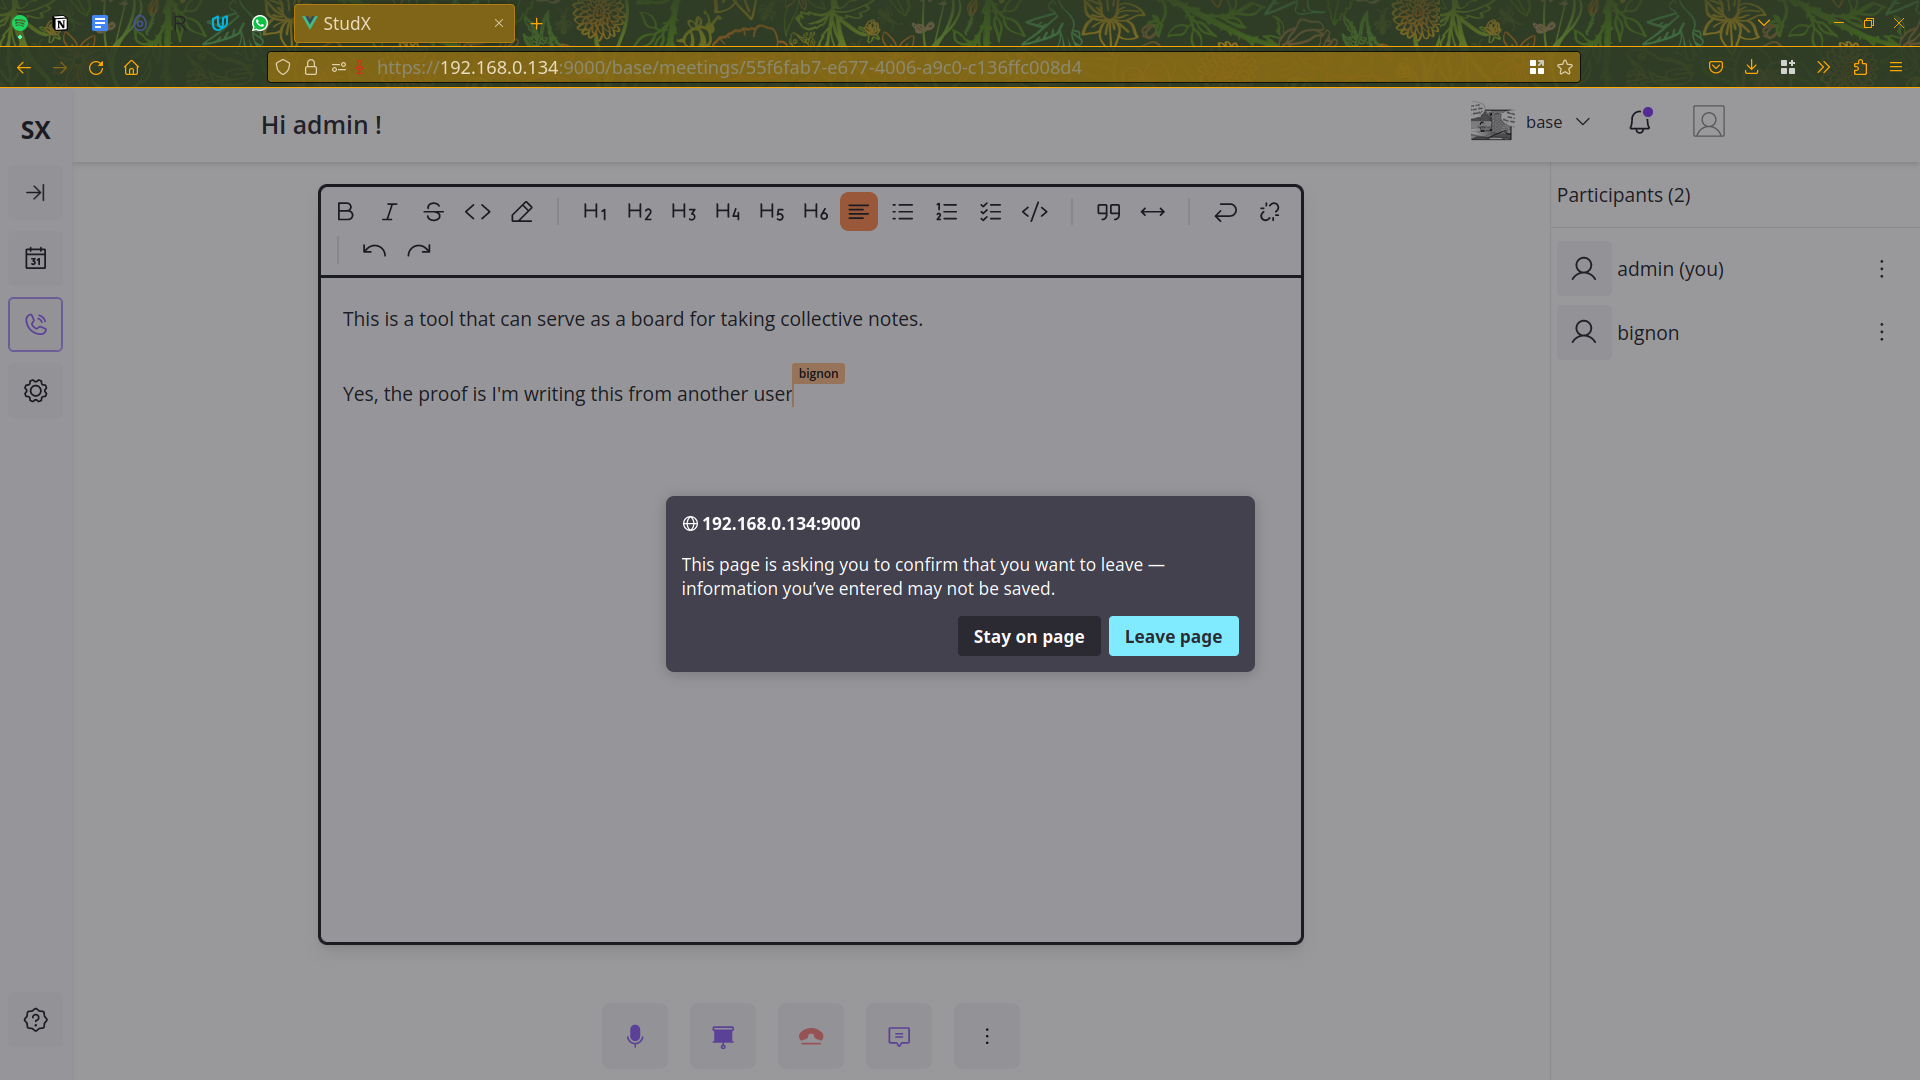
\includegraphics[width=\linewidth]{prototype/confirm-exit}}
      \caption{Confirmation de déconnexion}
  \end{subfigure}
  \vskip\baselineskip
  \begin{subfigure}[b]{\textwidth}
      \centering
      \frame{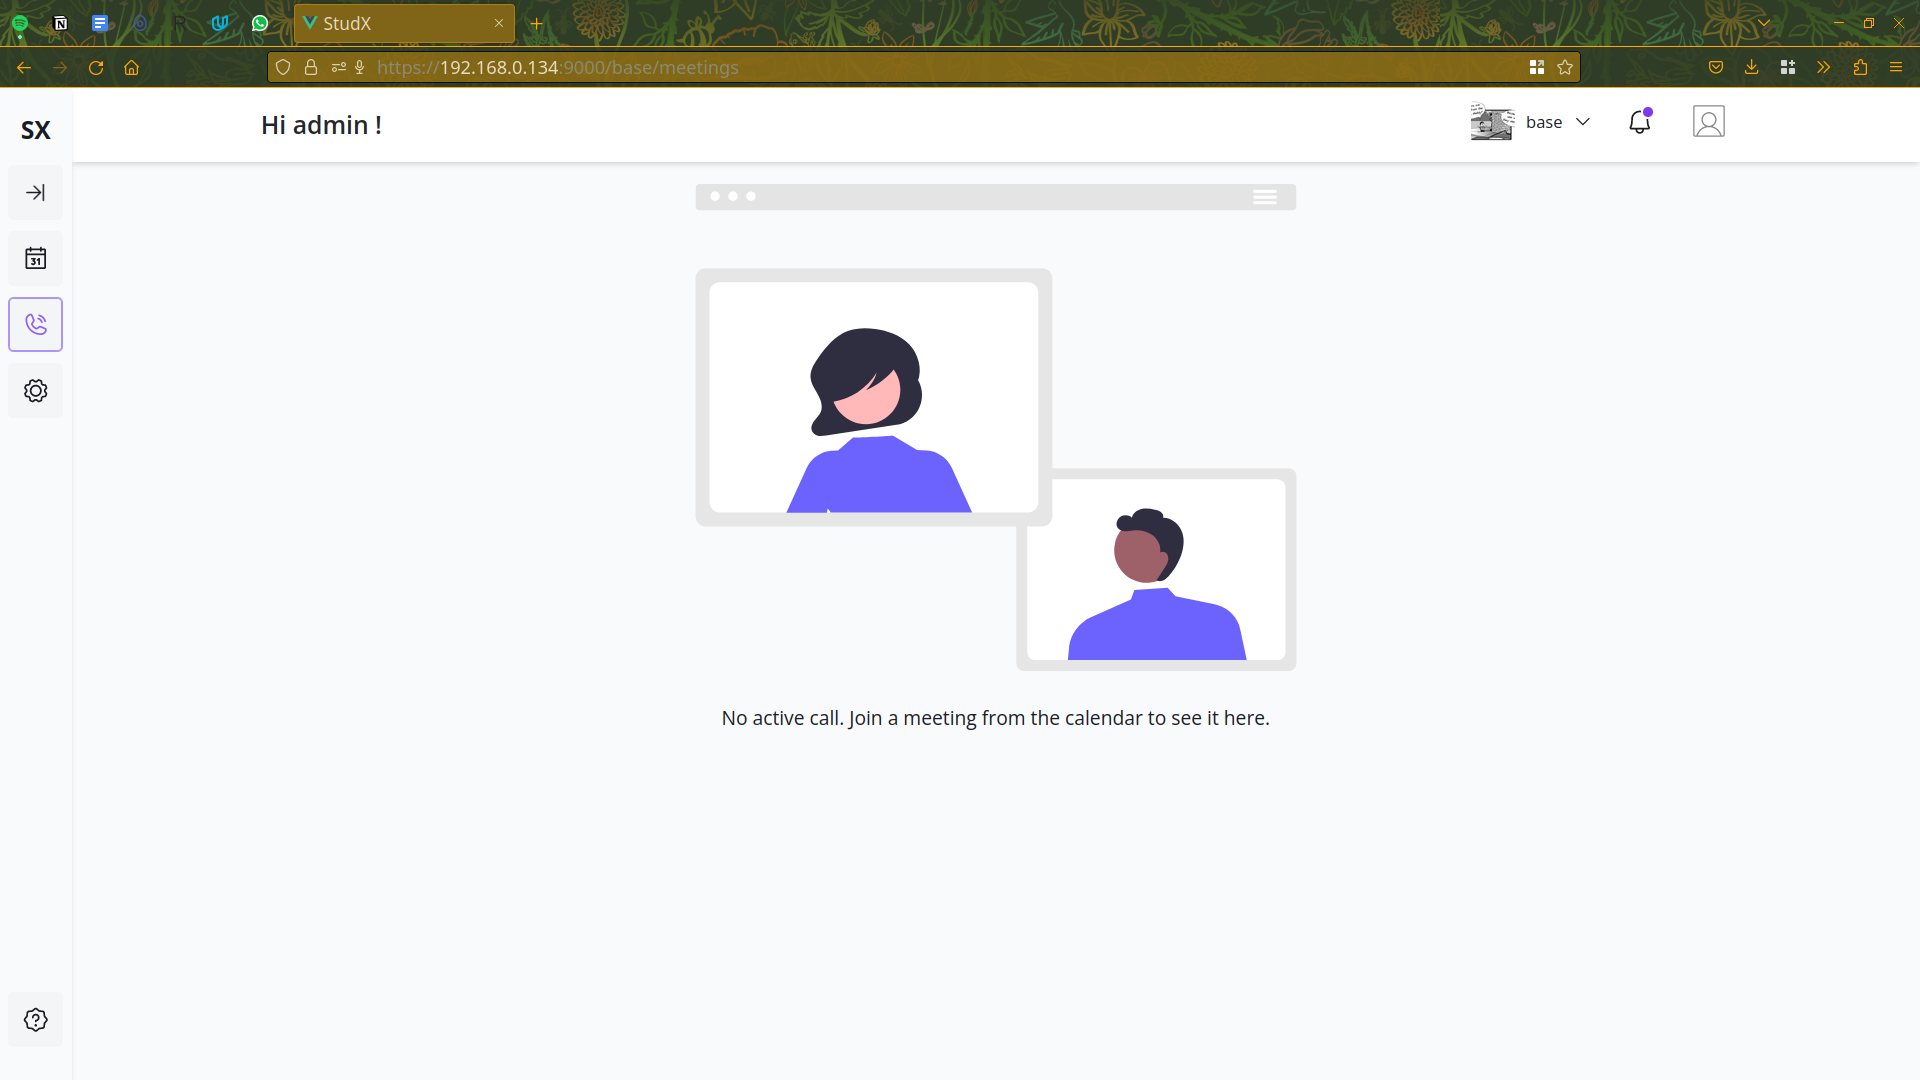
\includegraphics[width=\linewidth]{prototype/no-active-call}}
      \caption{Page de redirection après déconnexion}
  \end{subfigure}
  \caption{Processus de déconnexion.}
  \label{fig:exit}
\end{figure}

\subsection{Autres fonctionnalités}
Dans le but d'améliorer l'expérience utilisateur, nous avons jugé utile d’ajouter quelques fonctionnalités outre celles initialement visées. 
Parmi elles figurent le mode sombre et la mise en place d’un tutoriel interactif expliquant les diverses composantes de notre application. 

\begin{figure}[H]
  \centering
  \frame{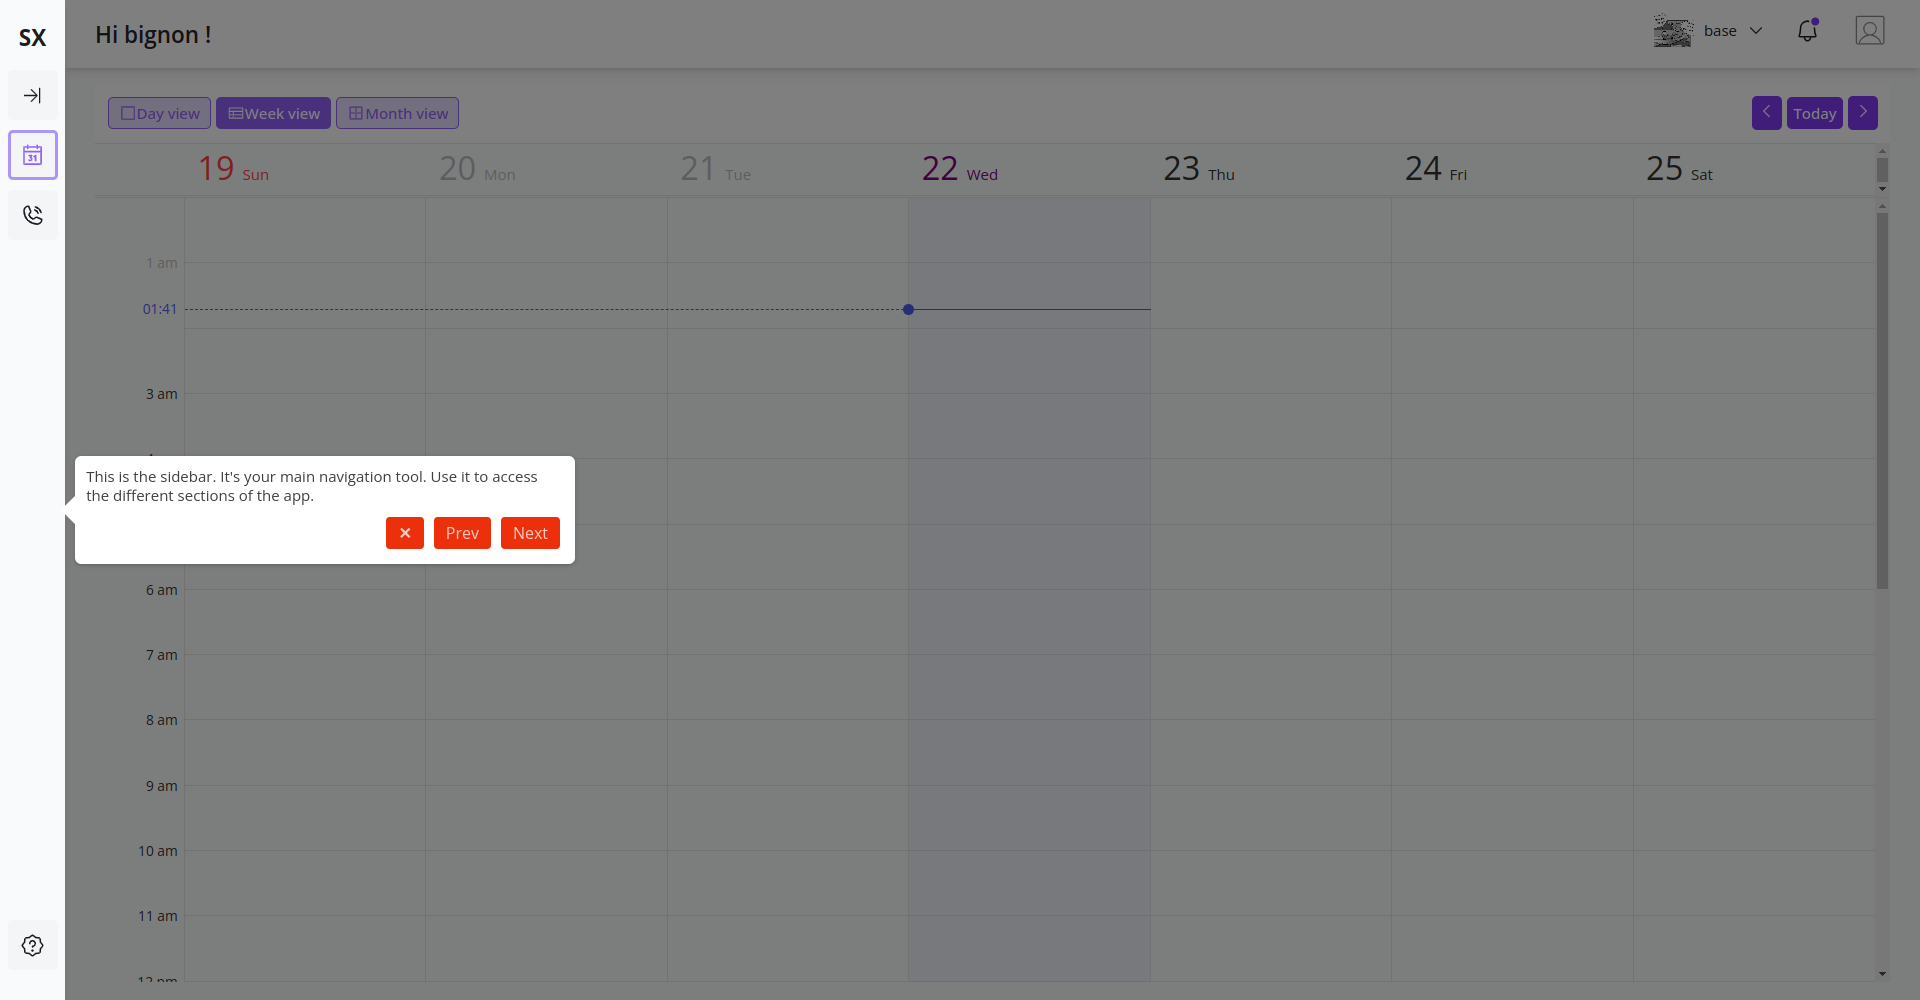
\includegraphics[width=\linewidth]{prototype/user-onboarding}}
  \caption{Tutoriel interactif d’introduction à StudX}
  \label{fig:onboarding}
\end{figure}


\begin{figure}[H]
  \centering
  \frame{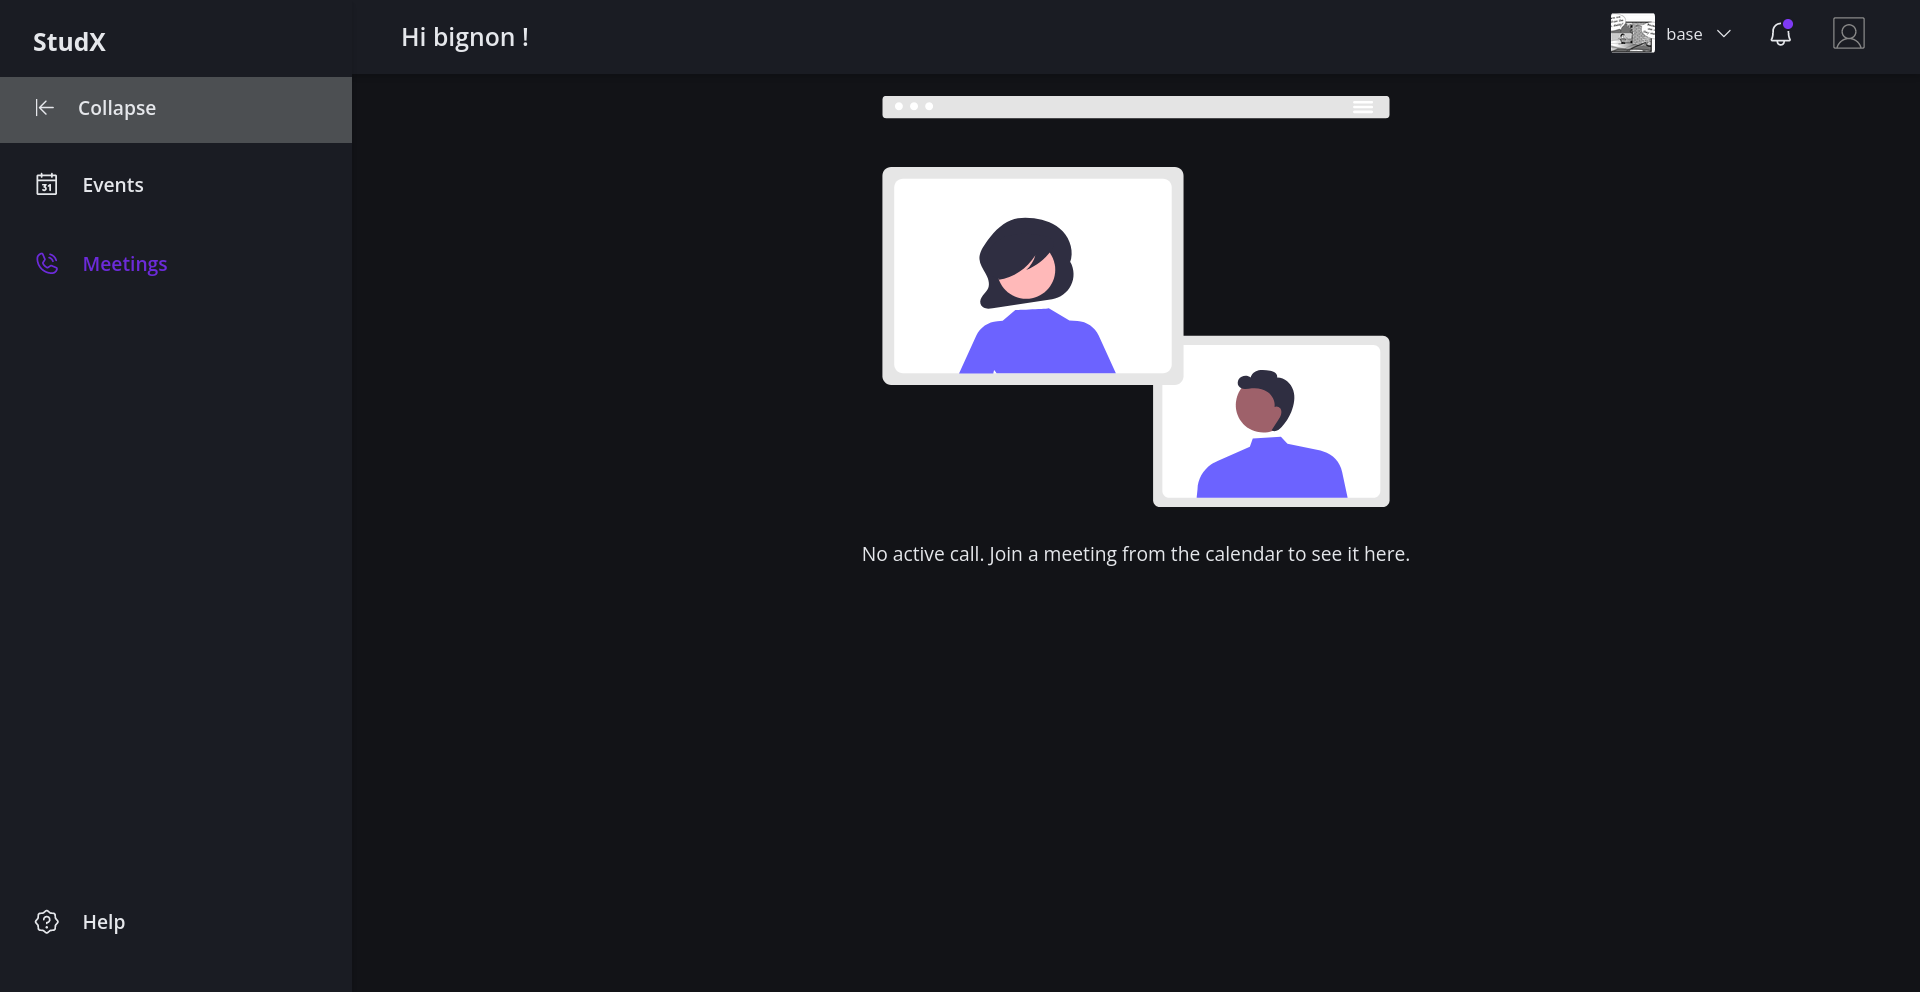
\includegraphics[width=\linewidth]{prototype/wip-dark-mode}}
  \caption{Mode sombre}
  \label{fig:dark_mode}
\end{figure}

Les administrateurs de la plateforme disposent également d’un accès aux paramètres de 
l'organisation qu’ils dirigent et peuvent ainsi ajouter ou retirer des membres (figure \ref{fig:settings}).

\begin{figure}[H]
  \centering
  \begin{subfigure}[b]{\textwidth}
      \centering
      \frame{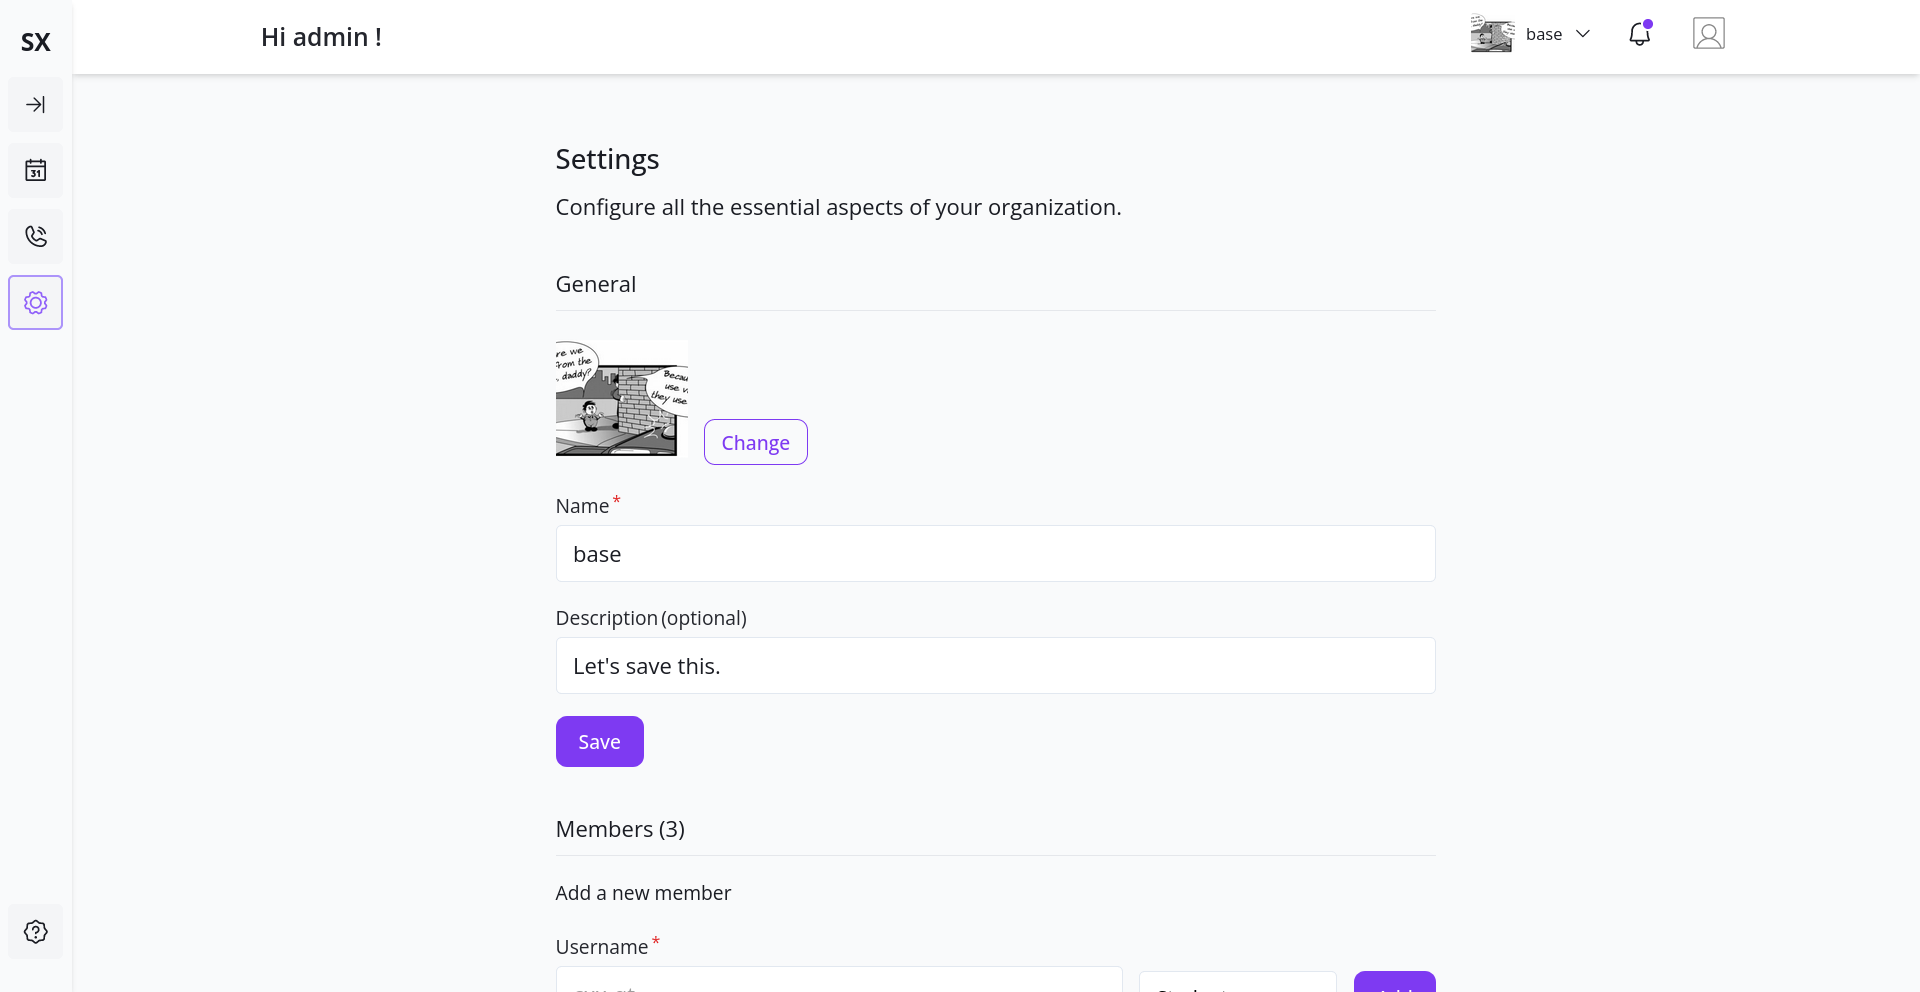
\includegraphics[width=\linewidth]{prototype/settings}}
      \caption{Paramètres généraux.}
  \end{subfigure}
  \vskip\baselineskip
  \begin{subfigure}[b]{\textwidth}
      \centering
      \frame{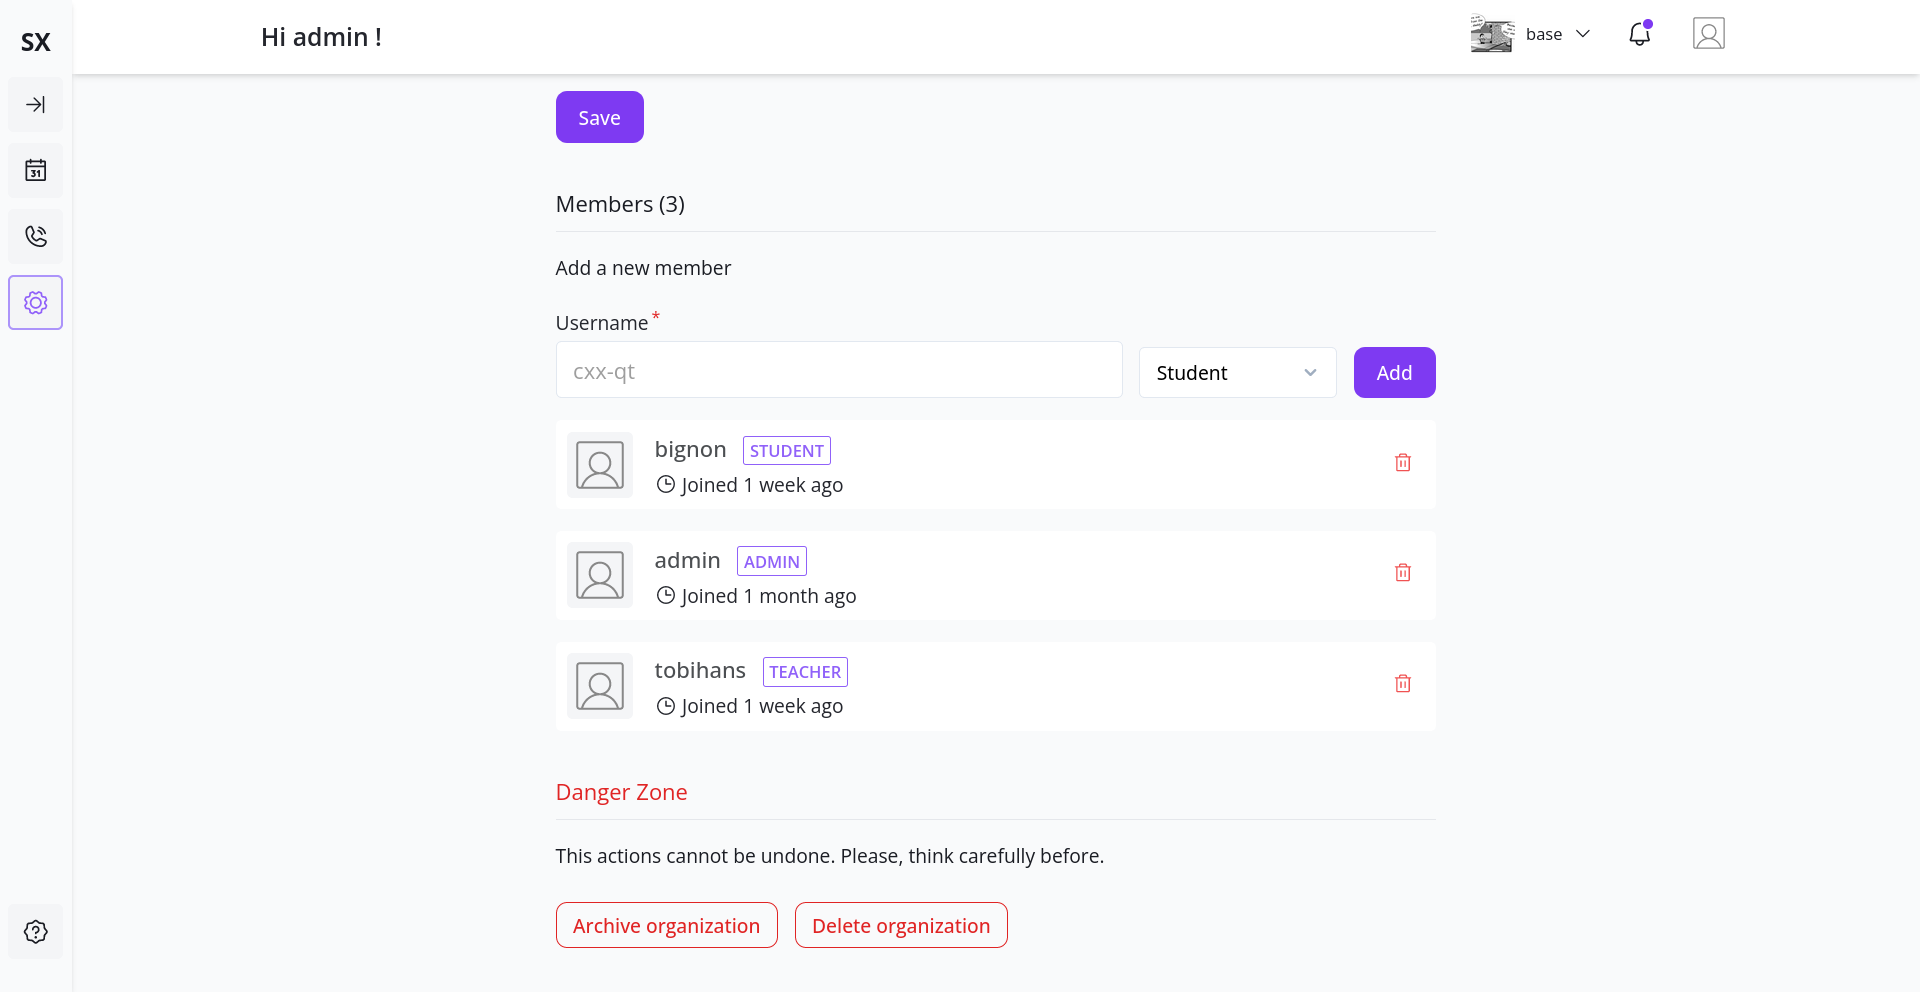
\includegraphics[width=\linewidth]{prototype/settings-end}}
      \caption{Gestion des membres.}
  \end{subfigure}
  \caption{Paramètres d'une organisation.}
  \label{fig:settings}
\end{figure}

\section{Discussion}
Le développement de l'application StudX a été un projet ambitieux, 
nécessitant la mise en place de nombreuses technologies modernes pour 
répondre aux besoins d'un environnement en ligne en constante évolution. 
Les fonctionnalités prévues pour l'application ont toutes été implémentées, 
permettant une tenue efficace de classes virtuelles en temps réel.

Cependant, la mise en œuvre de la technologie WebRTC a été un défi technique majeur 
tout au long du processus de développement. Le recours à cette technologie nécessite
une compréhension approfondie de son fonctionnement, ainsi que des compétences en 
programmation avancées pour l'adapter à nos besoins spécifiques. Cela a été rendu 
encore plus complexe par le fait que WebRTC est une technologie relativement nouvelle, 
qui ne cesse de se développer.


En outre, l'utilisation de code Open Source dans l'application a été également un facteur clé. 
Il a fallu comprendre le fonctionnement du code et le modifier pour répondre aux exigences de notre projet. 
Cela a nécessité un travail minutieux, impliquant une analyse approfondie du code existant, ainsi 
que des compétences en programmation avancées pour le modifier efficacement.

Malgré ces défis et bien d'autres, notre prototype est en place. Le choix du moteur Mediasoup pour les besoins de relais a été un choix judicieux. 
Ce moteur supporte un grand nombre de participants et intègre un concept de routeur pouvant supporter jusqu'à 500 personnes. 
Les routeurs peuvent également être connectés entre eux, offrant une grande évolutivité et une flexibilité pour répondre aux besoins futurs de l'application.
Le choix de s'abstenir de diffuser les flux vidéo permet également d'alléger le traffic et va permettre le support d'un grand nombre.

Le développement de StudX a été une expérience enrichissante. 
Bien que des défis aient été rencontrés tout au long du processus, 
l'application fonctionne maintenant et répond aux objectifs initialement fixés.

\section*{Conclusion}
Après la conception et le développement de l'application, il est clair que le prototype répond aux besoins identifiés et remplit les objectifs fixés pour ce projet. 
Les tests effectués ont démontré la fiabilité et la performance de l'application, ainsi que sa capacité à gérer les fonctionnalités attendues. 
Cependant, cela ne signifie pas qu'elle est parfaite, car de nombreux aspects peuvent être encore améliorés et développés pour répondre à des besoins futurs ou pour satisfaire des demandes plus spécifiques. 